% --- impostazione documento  ----------------------------------------
\documentclass[12pt,a4paper,twoside]{report}  % twoside per stampa fronte e retro

% --- impostazione pagina ----------------------------------------
\usepackage[
  a4paper,
  left=2.5cm,  %INNER E OUTER SE SI STAMPA, DA DIFFERENZIARE
  right=2.5cm, 
  top=3cm,
  bottom=2cm
]{geometry}

% --- encoding e font ---------------------------------------- (Basati su compilatore pdfLatex)
\usepackage[utf8]{inputenc}     % UTF‑8 input
\usepackage[T1]{fontenc}        % font encoding
\usepackage{newtxtext,newtxmath}% Times‑like text + matematica in stile Times
\usepackage{needspace}
\usepackage{etoolbox}
\widowpenalty=10000   % non lasciare righe isolate in cima pagina
\clubpenalty=10000    % non lasciare righe isolate in fondo pagina
\sloppy

% --- altri pacchetti ---------------------------------------
\usepackage[italian]{babel}
\usepackage{amsmath}            % opzionale, newtxmath carica già amsmath
\usepackage{graphicx,wrapfig,float,booktabs,siunitx}
\usepackage{url}
\usepackage[version=4]{mhchem}
\usepackage{microtype}
\usepackage{setspace}
\usepackage{caption}
\usepackage{subcaption}
\usepackage{pdflscape}
\usepackage{fancyhdr}
\usepackage{lscape}
\usepackage{hyperref}
\usepackage{afterpage}
\setstretch{1.2}        % imposta interlinea 1.2 per tutto il documento

% --- controllo automatico generazione nuove pagine ---------------------------------------
% Quanti “baselineskip” (righe) minimi servono:
\newcommand{\ChapterSpace}{15\baselineskip}
\newcommand{\SectionSpace}{8\baselineskip}
\newcommand{\SubsectionSpace}{6\baselineskip}

% Prima di ogni capitolo/sezione... forza il controllo
\preto\chapter     {\Needspace{\ChapterSpace}}
\preto\section     {\Needspace{\SectionSpace}}
\preto\subsection  {\Needspace{\SubsectionSpace}}
\preto\subsubsection {\Needspace{4\baselineskip}}  % se usi subsub

% --- directory immagini ----------------------------------------
\graphicspath{{Images/}}      % Percorso di default per le immagini

% --- gerarchia titoli SPECIFICA PER FORMATO REPORT  ---------------------------------------
%\chapter{Capitolo Uno}            
%\section{Prima Sezione}           % 1.1
%\subsection{Prima Sottosezione}   % 1.1.1
%\subsubsection{Primo Livello 3}   % 1.1.1.1
%\paragraph{Paragrafo}             % 1.1.1.1.1
%\subparagraph{Sottoparag.}        % 1.1.1.1.1.1

% --- Inizio documento e prima pagina  ---------------------------------------
\begin{document}
\begin{titlepage}
  \centering

  {\small
    Università degli Studi di Modena e Reggio Emilia\\
    Dipartimento di Scienze e Metodi dell'Ingegneria
  }\\[1cm]
  {\Large Corso di Laurea in Ingegneria Meccatronica}\\[2cm]

  \vfill
  {\Huge\bfseries Five Strokes Engine(ers)}\\[1em]
  {\Huge\bfseries Mecha Pitters}\\[1em]
  \vfill

  \begin{minipage}[t]{0.45\textwidth}
    \raggedright
    \textbf{A cura di:}\\
    Bonacini Alex\\
    Bortolotti Riccardo\\
    Cintoli Salvatore\\
    Corradi Matteo\\ 
    Grisendi Matteo
    
  \end{minipage}%
  \hfill
  \vspace{2cm}

  {\small Anno Accademico 2024/2025}
\end{titlepage}

% --- Indice, indice figure, indice tabelle  ---------------------------------------
\renewcommand{\contentsname}{Indice}
\tableofcontents
\newpage
\listoffigures
\newpage
\listoftables

% --- Inizio del testo  ---------------------------------------
\chapter{ Pianificazione di prodotto}
Il processo di progettazione e realizzazione di un prodotto innovativo consta di diverse fasi, prima fra tutte la pianificazione di prodotto. La pianificazione di prodotto inizia con l'analisi delle opportunità e termina con la dichiarazione di intenti. L'analisi delle opportunità identifica un portfolio di prodotti nel quale si identifica la possibilità di inserire un prodotto innovativo. 
\begin{figure}[H] %[H] serve a forzare l'immagine nella posizione devo metto il codice
    \centering
    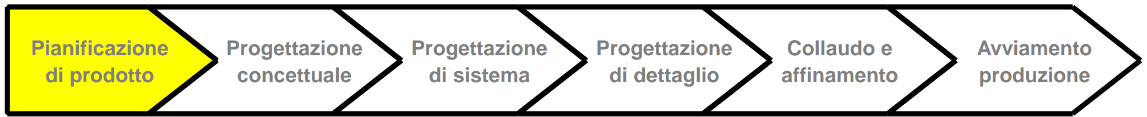
\includegraphics[width=1\linewidth]{pianificazioneProdotto.png}
    \label{fig:pianificazioneProdotto}
\end{figure}
Una volta definito il portfolio prodotti nel quale inserire il prodotto che sarà oggetto di progettazione, si allocano le risorse aziendali, si definiscono le tempistiche di sviluppo (tramite il diagramma di Gantt, rappresentato in Figura \ref{fig:ganttModificato}) e si formula la dichiarazione di intenti.
\section{Dichiarazione di intenti e Diagramma di Gantt}
Segue la dichiarazione di intenti per il prodotto MechaPitter.

\textbf{Descrizione:} Un elettrodomestico automatico, alimentato e portatile, per denocciolare frutti di piccole dimensioni.

\textbf{Obiettivi:}
\begin{itemize}
\item TTM (Time To Market, ossia tempo di lancio del prodotto sul mercato) inferiore a 9 mesi;
\item Prezzo di vendita inferiore o uguale a 80 €;
\item Produzione prevista di 10.000 esemplari/anno;
\item Margine lordo del 25%.
\end{itemize}

\textbf{Mercato:}
\begin{itemize}
\item Utenza domestica e commerciale;
\item Elettronica di consumo;
\item Ferramente;
\item Televendite.
\end{itemize}

\textbf{Ipotesi e vincoli:}
\begin{itemize}
\item Elabora tre differenti tipologie di frutti (ciliegie, olive e prugne);
\item È automatico;
\item È alimentato;
\item È senza fili;
\item Preserva al meglio l'integrità e le caratteristiche organolettiche dei frutti.
\end{itemize}

\textbf{Interessati:}
\begin{itemize}
\item Uso domestico (famiglie, ecc...);
\item Settore ristorazione (gelaterie, bar, pasticcerie);
\item Rivendite di elettrodomestici e casalinghi;
\item Ufficio vendite e servizio assistenza.
\end{itemize}

Segue il diagramma di Gantt adattato alle esigenze degli studenti del gruppo Five Strokes Engine(ers)

\newpage
\begin{landscape}
%\thispagestyle{empty} % x rimuovere numero pagina
\begin{figure}
    \centering
    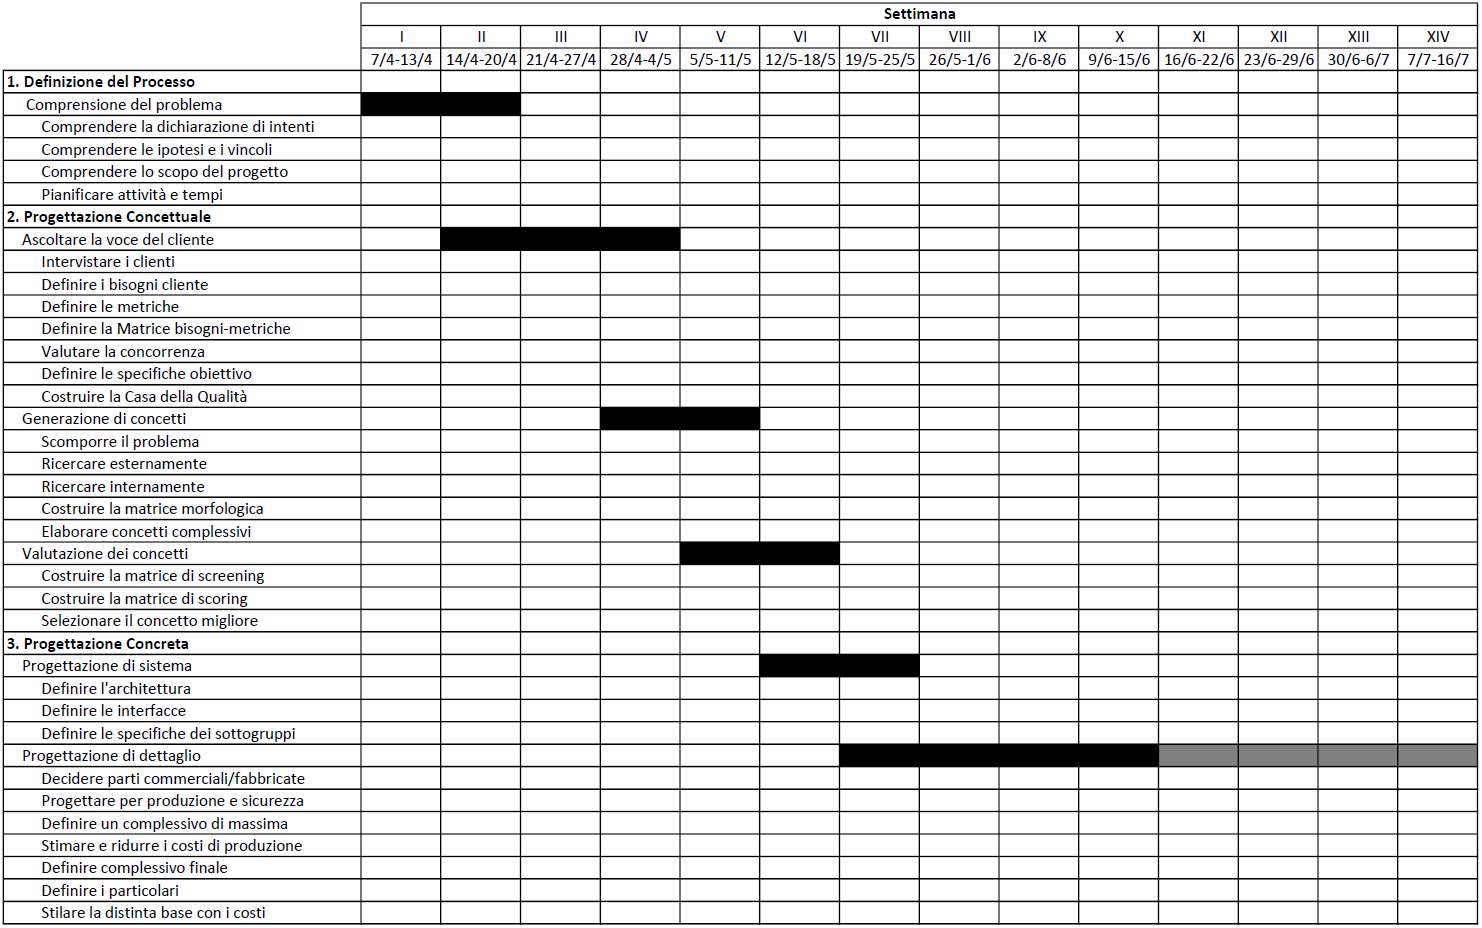
\includegraphics[width=1\linewidth]{ganttModificato.png}
    \caption{Diagramma di Gantt}
    \label{fig:ganttModificato}
\end{figure}
\end{landscape}
\newpage

\chapter{Progettazione concettuale}
La progettazione concettuale è una fase del processo di progettazione di un prodotto che si basa sulla dichiarazione d'intenti precedentemente formulata per definire un concetto di prodotto. In particolare la progettazione concettuale è mirata all'individuazione dei bisogni cliente, sulla base dei quali si definiscono le specifiche obiettivo che il prodotto dovrà soddisfare. Successivamente si procede con la creazione della Casa della Qualità, con la generazione dei concetti di prodotto e relativa valutazione. Infine si seleziona un concetto campione e si definiscono le specifiche finali.
\begin{figure}[H] %[H] serve a forzare l'immagine nella posizione devo metto il codice
    \centering
    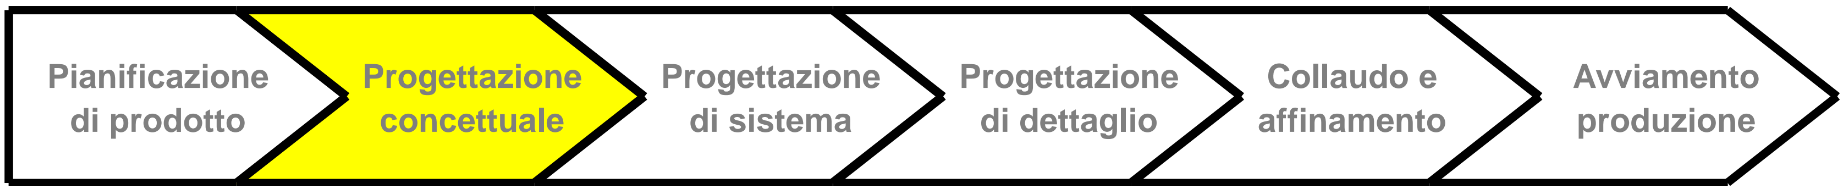
\includegraphics[width=1\linewidth]{progettazioneConcettuale.png}
    \label{fig:progettazioneConcettuale}
\end{figure}
\section{Identificazione e analisi dei bisogni cliente}
\label{sec:identificazioneBisogniCliente}
I bisogni cliente sono stati definiti sulla base dei risultati ottenuti da un sondaggio redatto mediante Google Form. Il sondaggio si è focalizzato sulla raccolta delle seguenti categorie di dati in una popolazione di 52 individui:
\begin{itemize}
\item Caratteristiche demografiche ed occupazionali della popolazione campionata;
\item Conoscenza, possibile ambito di utilizzo e frequenza di utilizzo di un denocciolatore automatico;
\item Tipologia di frutti di maggiore interesse e utilizzo specifico;
\item Definizione dei bisogni prioritari.
\end{itemize}
Dal sondaggio si evince che il 36,5\% dei votanti è interessato all'acquisto di un denocciolatore automatico e il 63,5\% ritiene che 60€-80€ sia una forbice di prezzo adeguata per questo prodotto.
I risultati del sondaggio sono riportati nei grafici seguenti.

\begin{figure}[htbp]
  \centering
  \begin{subfigure}[b]{0.45\textwidth}
    \centering
    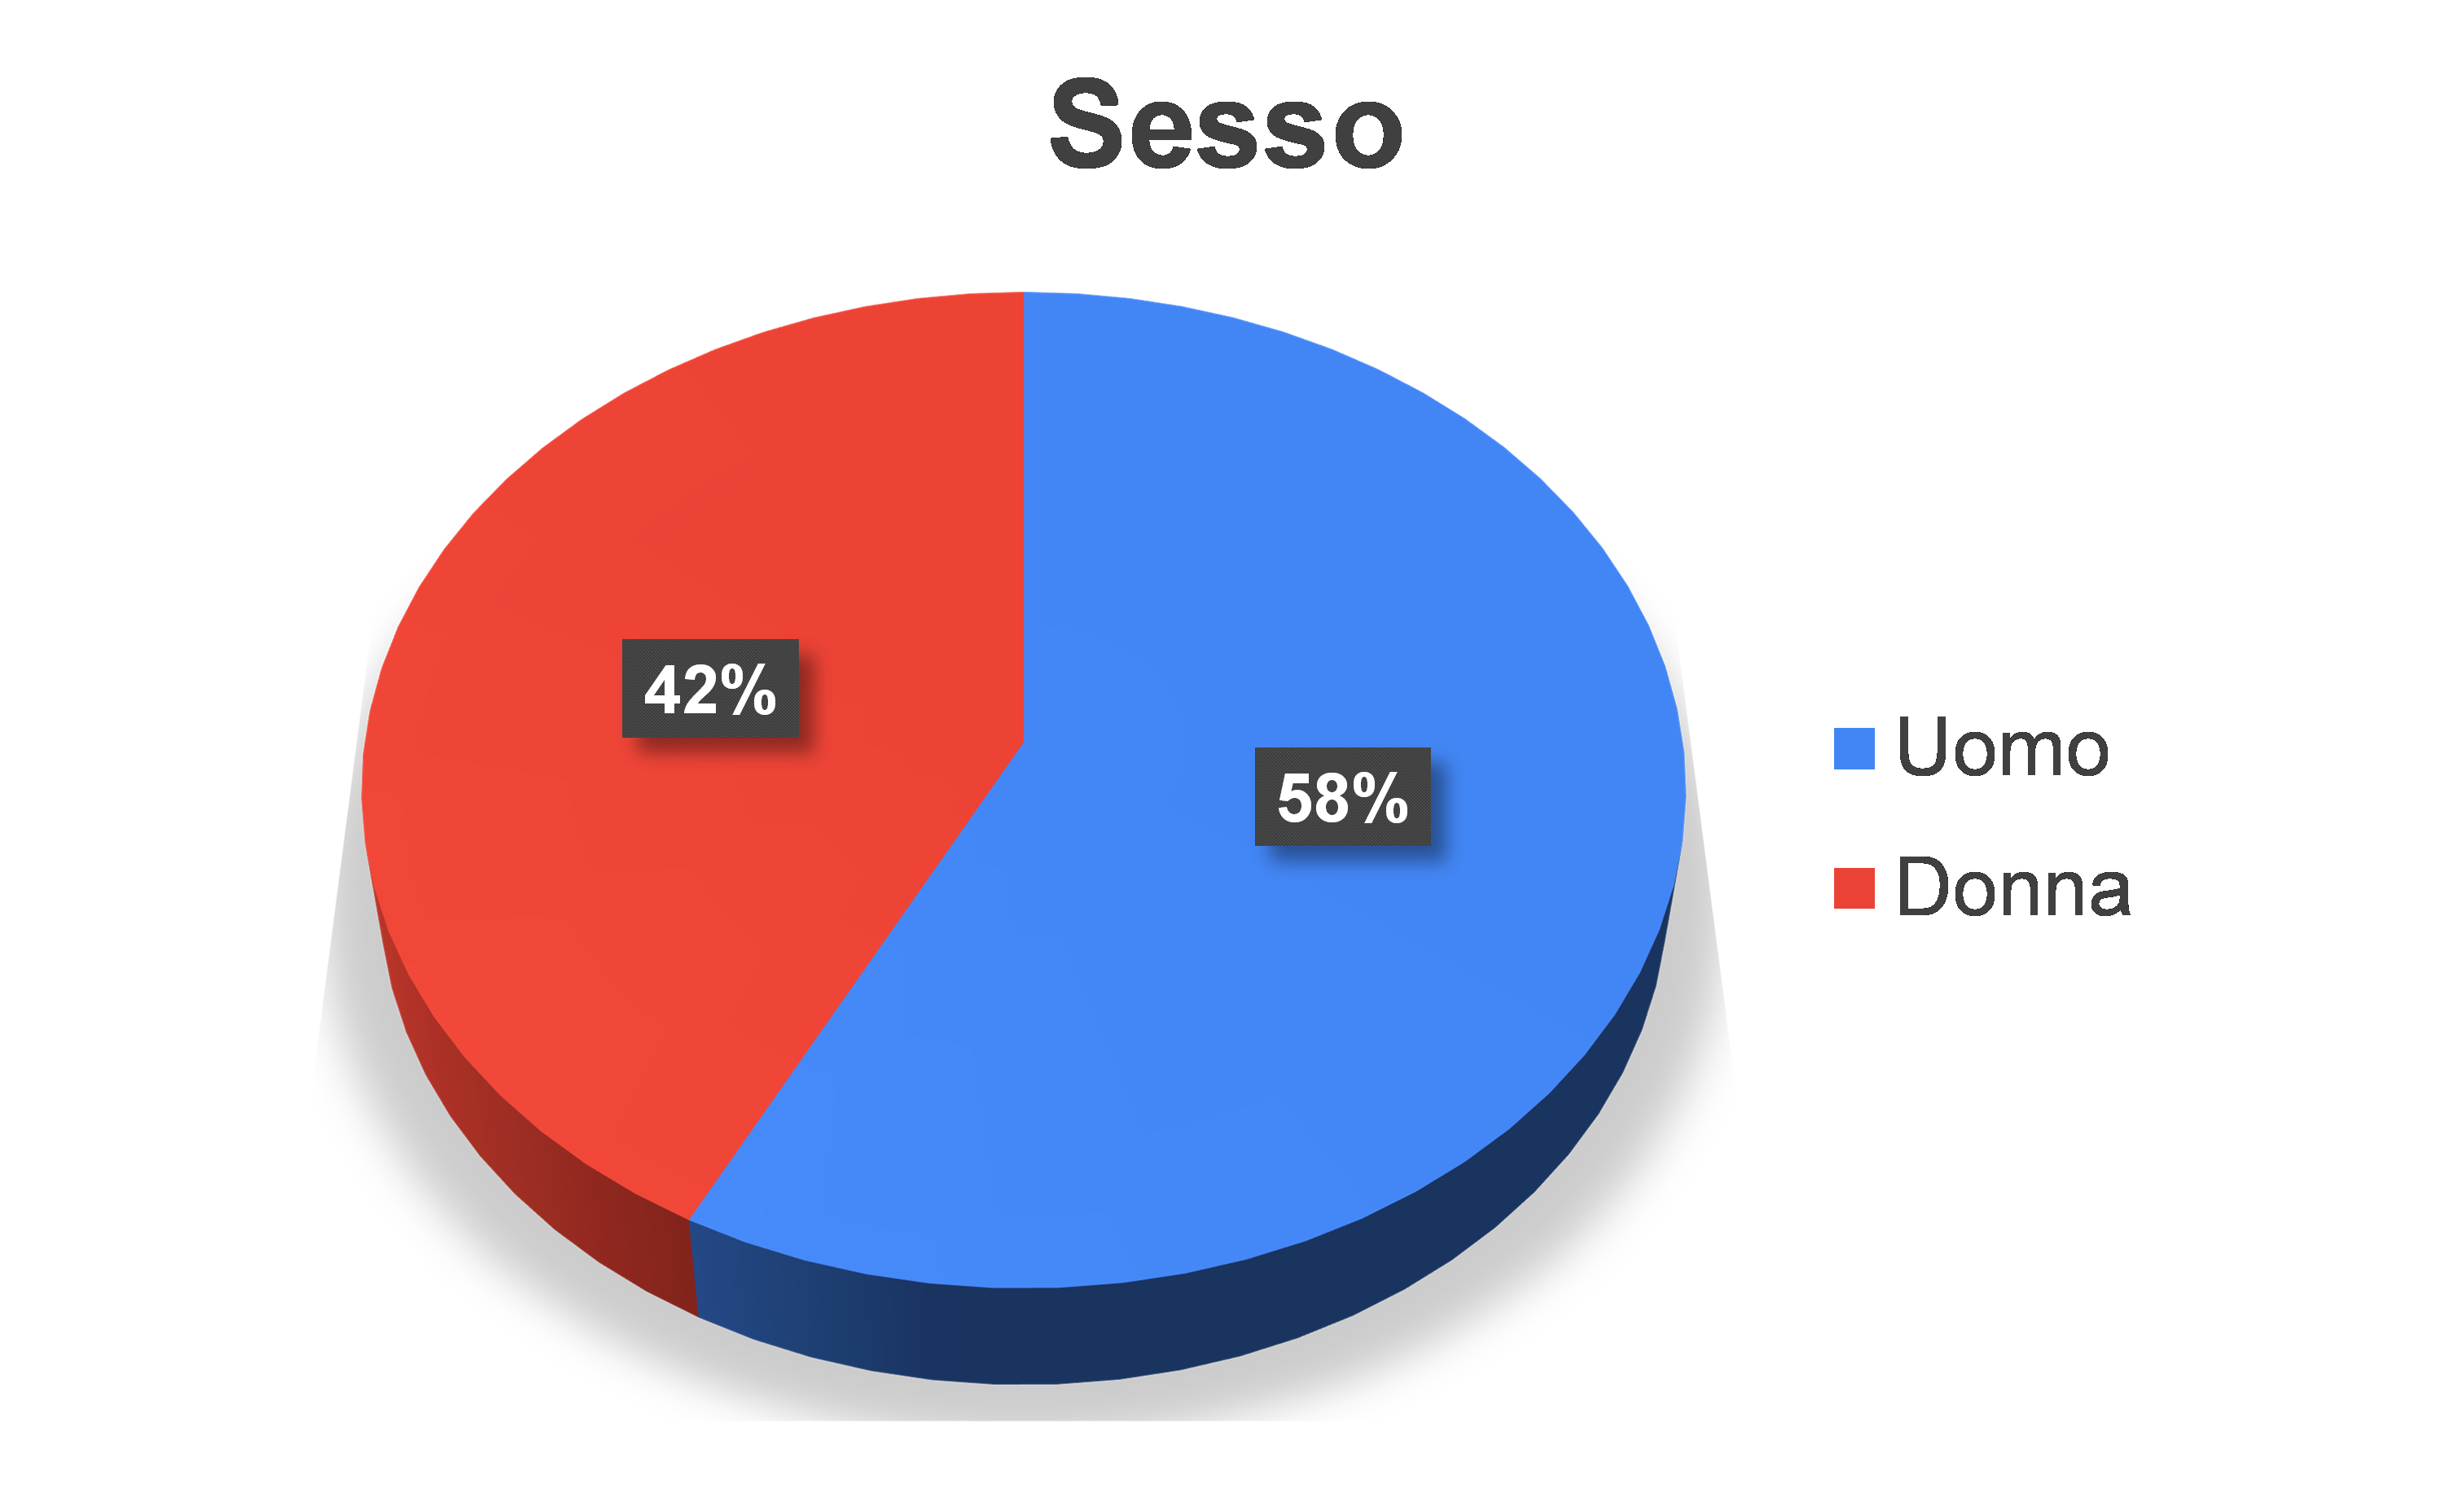
\includegraphics[width=\textwidth]{sesso.png}
    \caption{}
    \label{fig:sesso}
  \end{subfigure}
  \hfill
  \begin{subfigure}[b]{0.45\textwidth}
    \centering
    \includegraphics[width=\textwidth]{fasciaEtà.png}
    \caption{}
    \label{fig:fascia_eta}
  \end{subfigure}
  \vskip\baselineskip
  \begin{subfigure}[b]{0.45\textwidth}
    \centering
    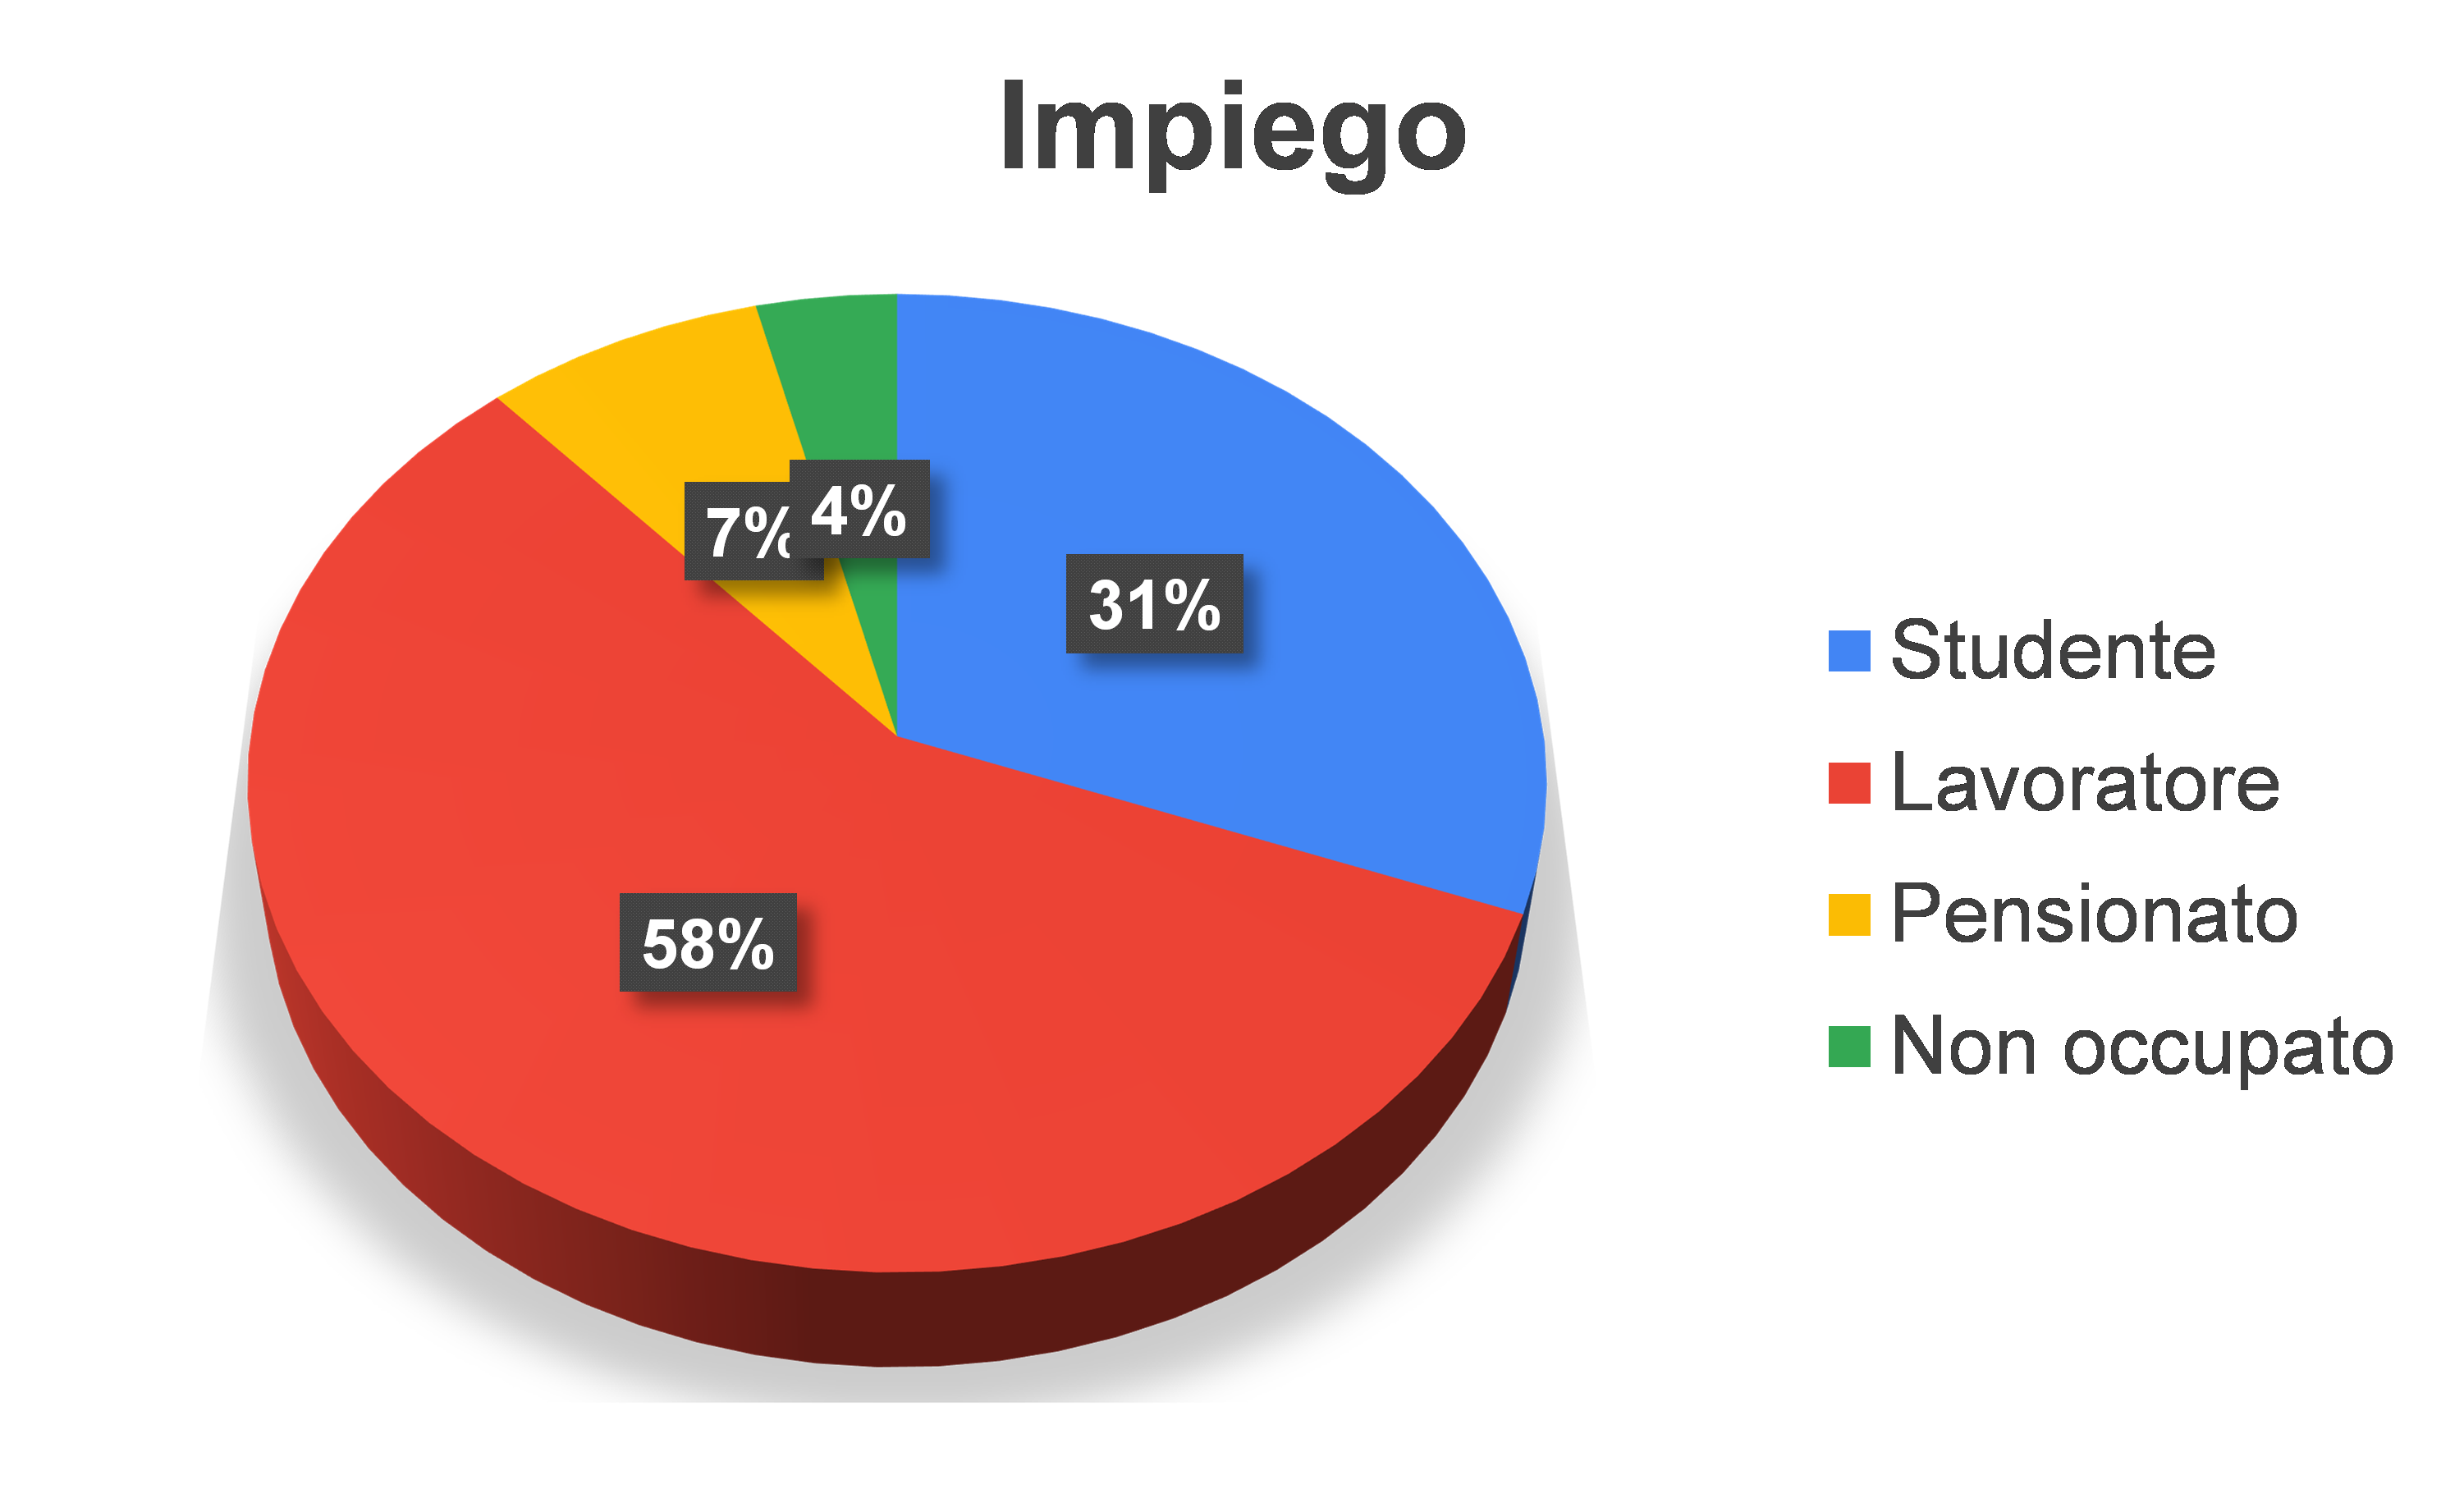
\includegraphics[width=\textwidth]{impiego.png}
    \caption{}
    \label{fig:impiego}
  \end{subfigure}
  \caption{Caratteristiche demografiche ed occupazionali della popolazione campionata}
  \label{fig:caratteristiche_demografiche}
\end{figure}

\begin{figure}[htbp]
  \centering
  \begin{subfigure}[b]{0.45\textwidth}
    \centering
    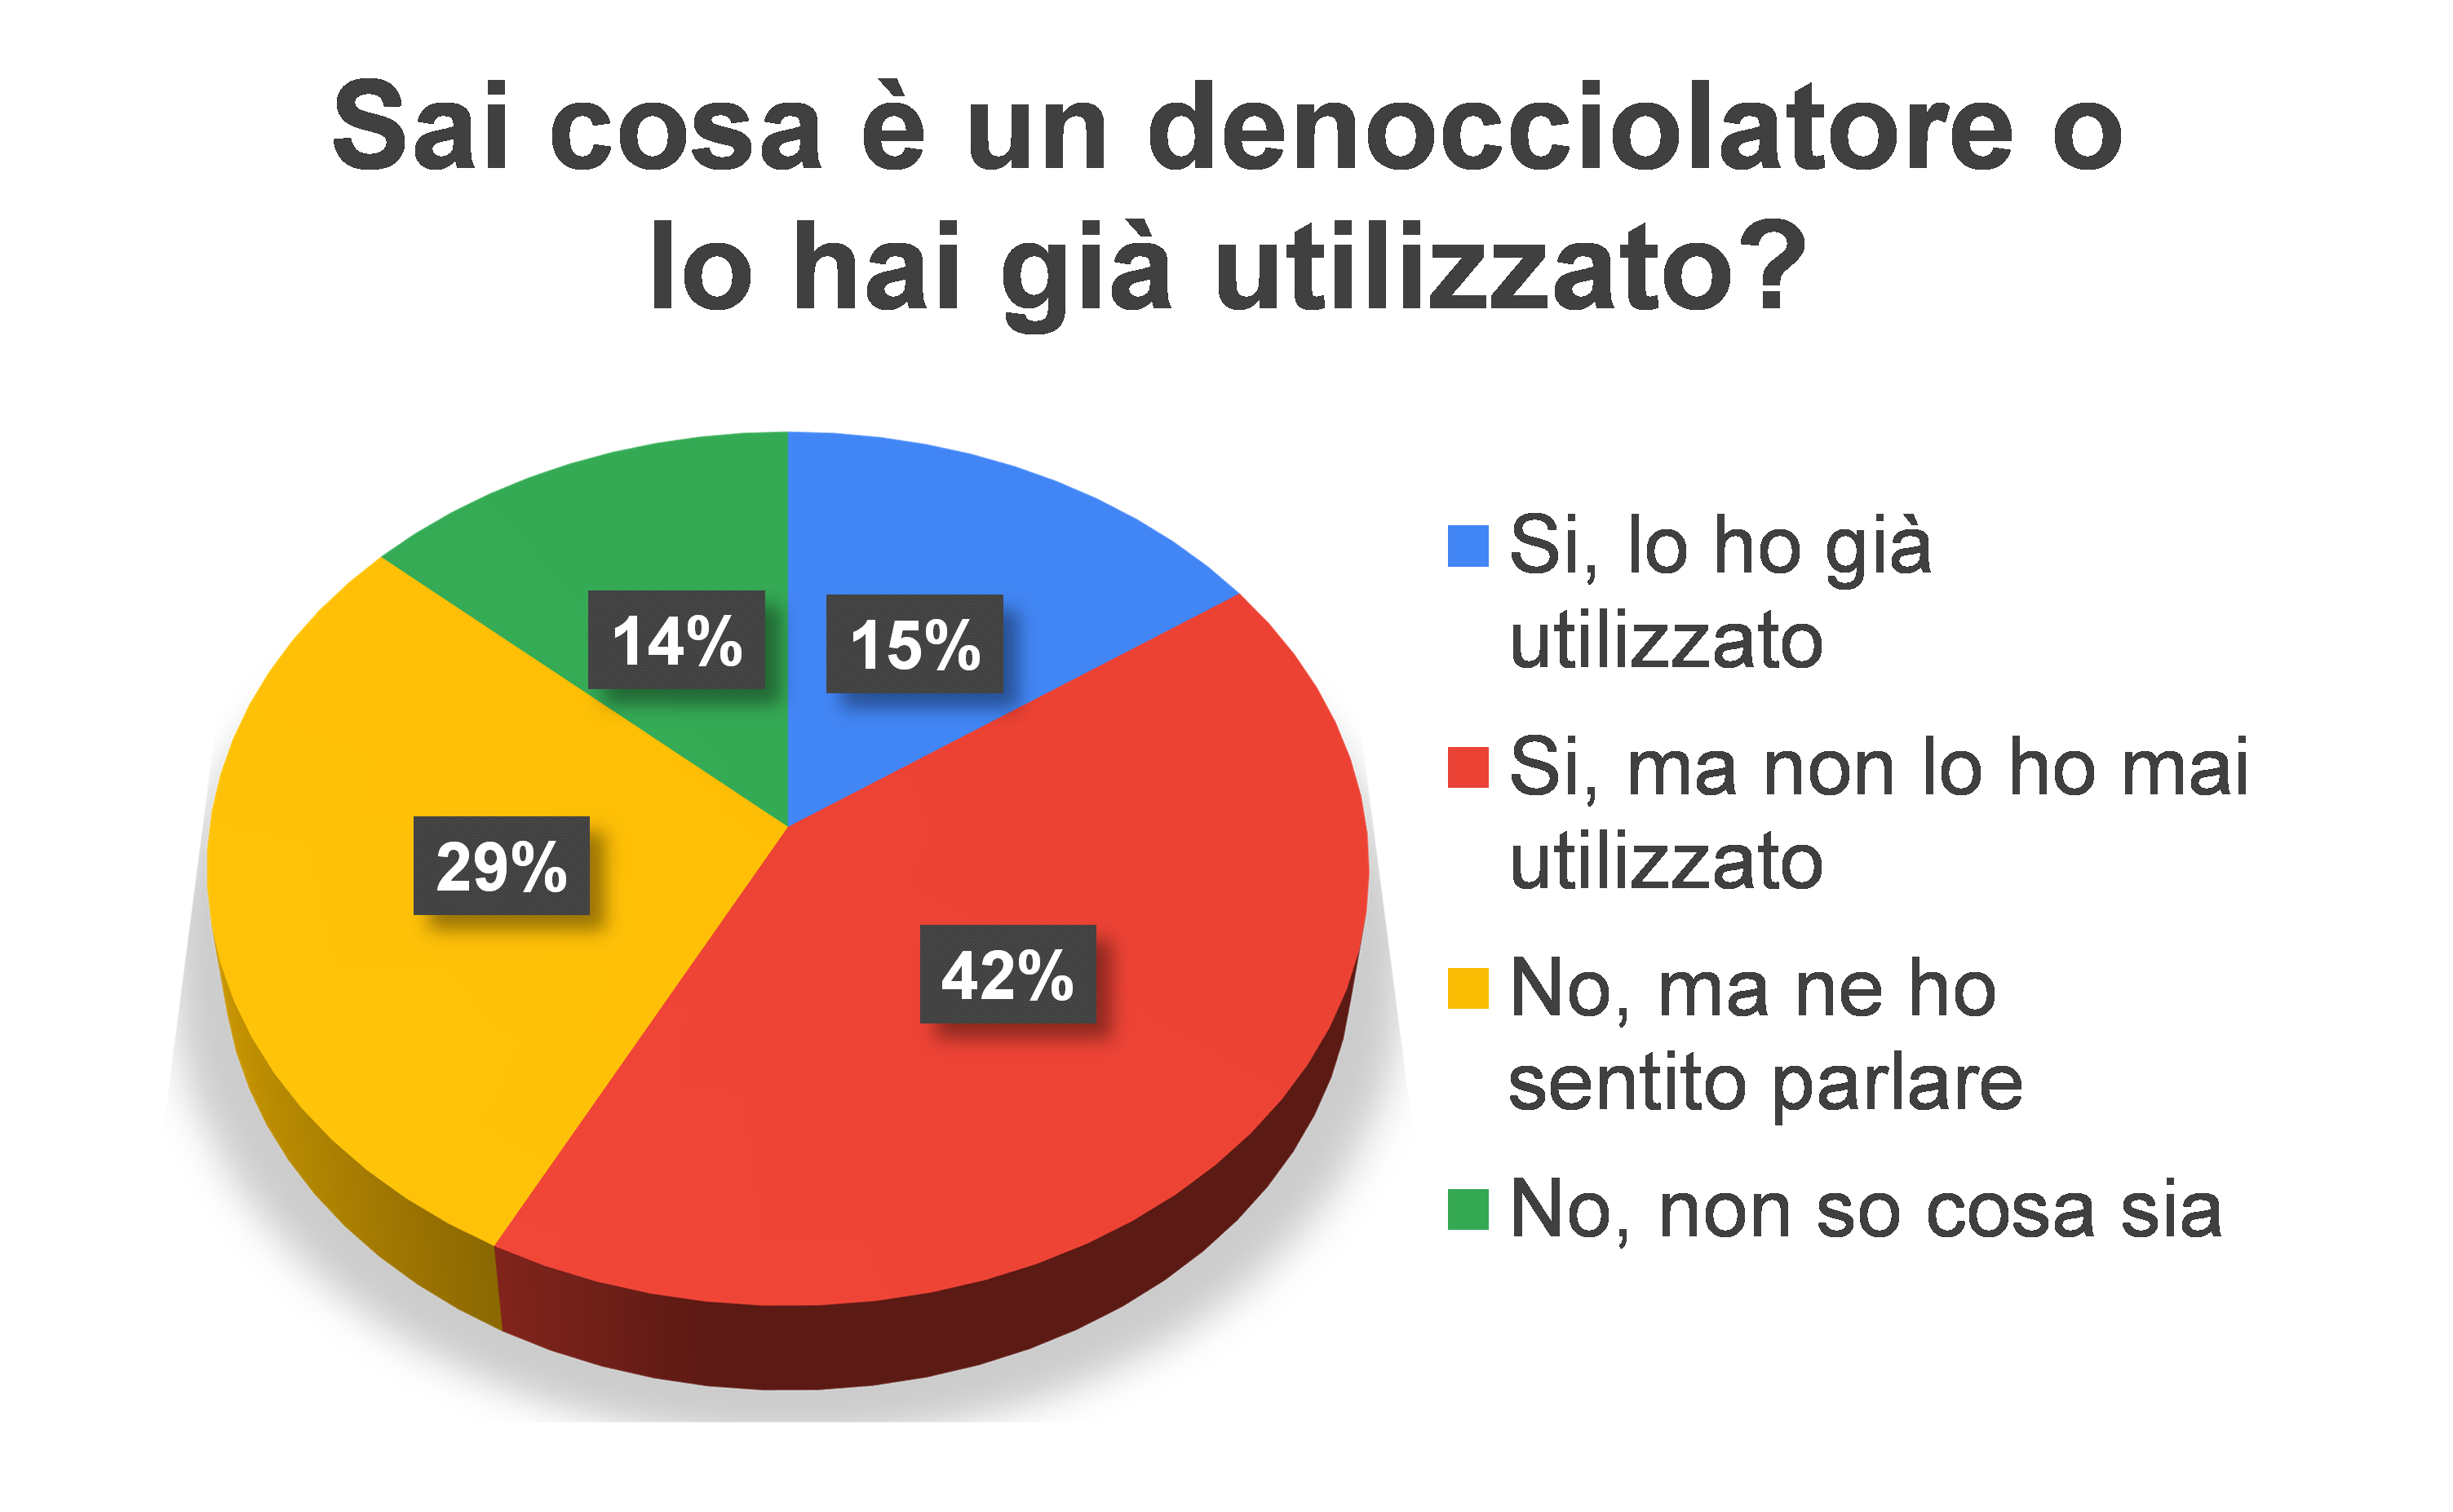
\includegraphics[width=\textwidth]{conoscenzaDenocciolatore.png}
    \caption{}
    \label{fig:conoscenza_denocciolatore}
  \end{subfigure}
  \hfill
  \begin{subfigure}[b]{0.45\textwidth}
    \centering
    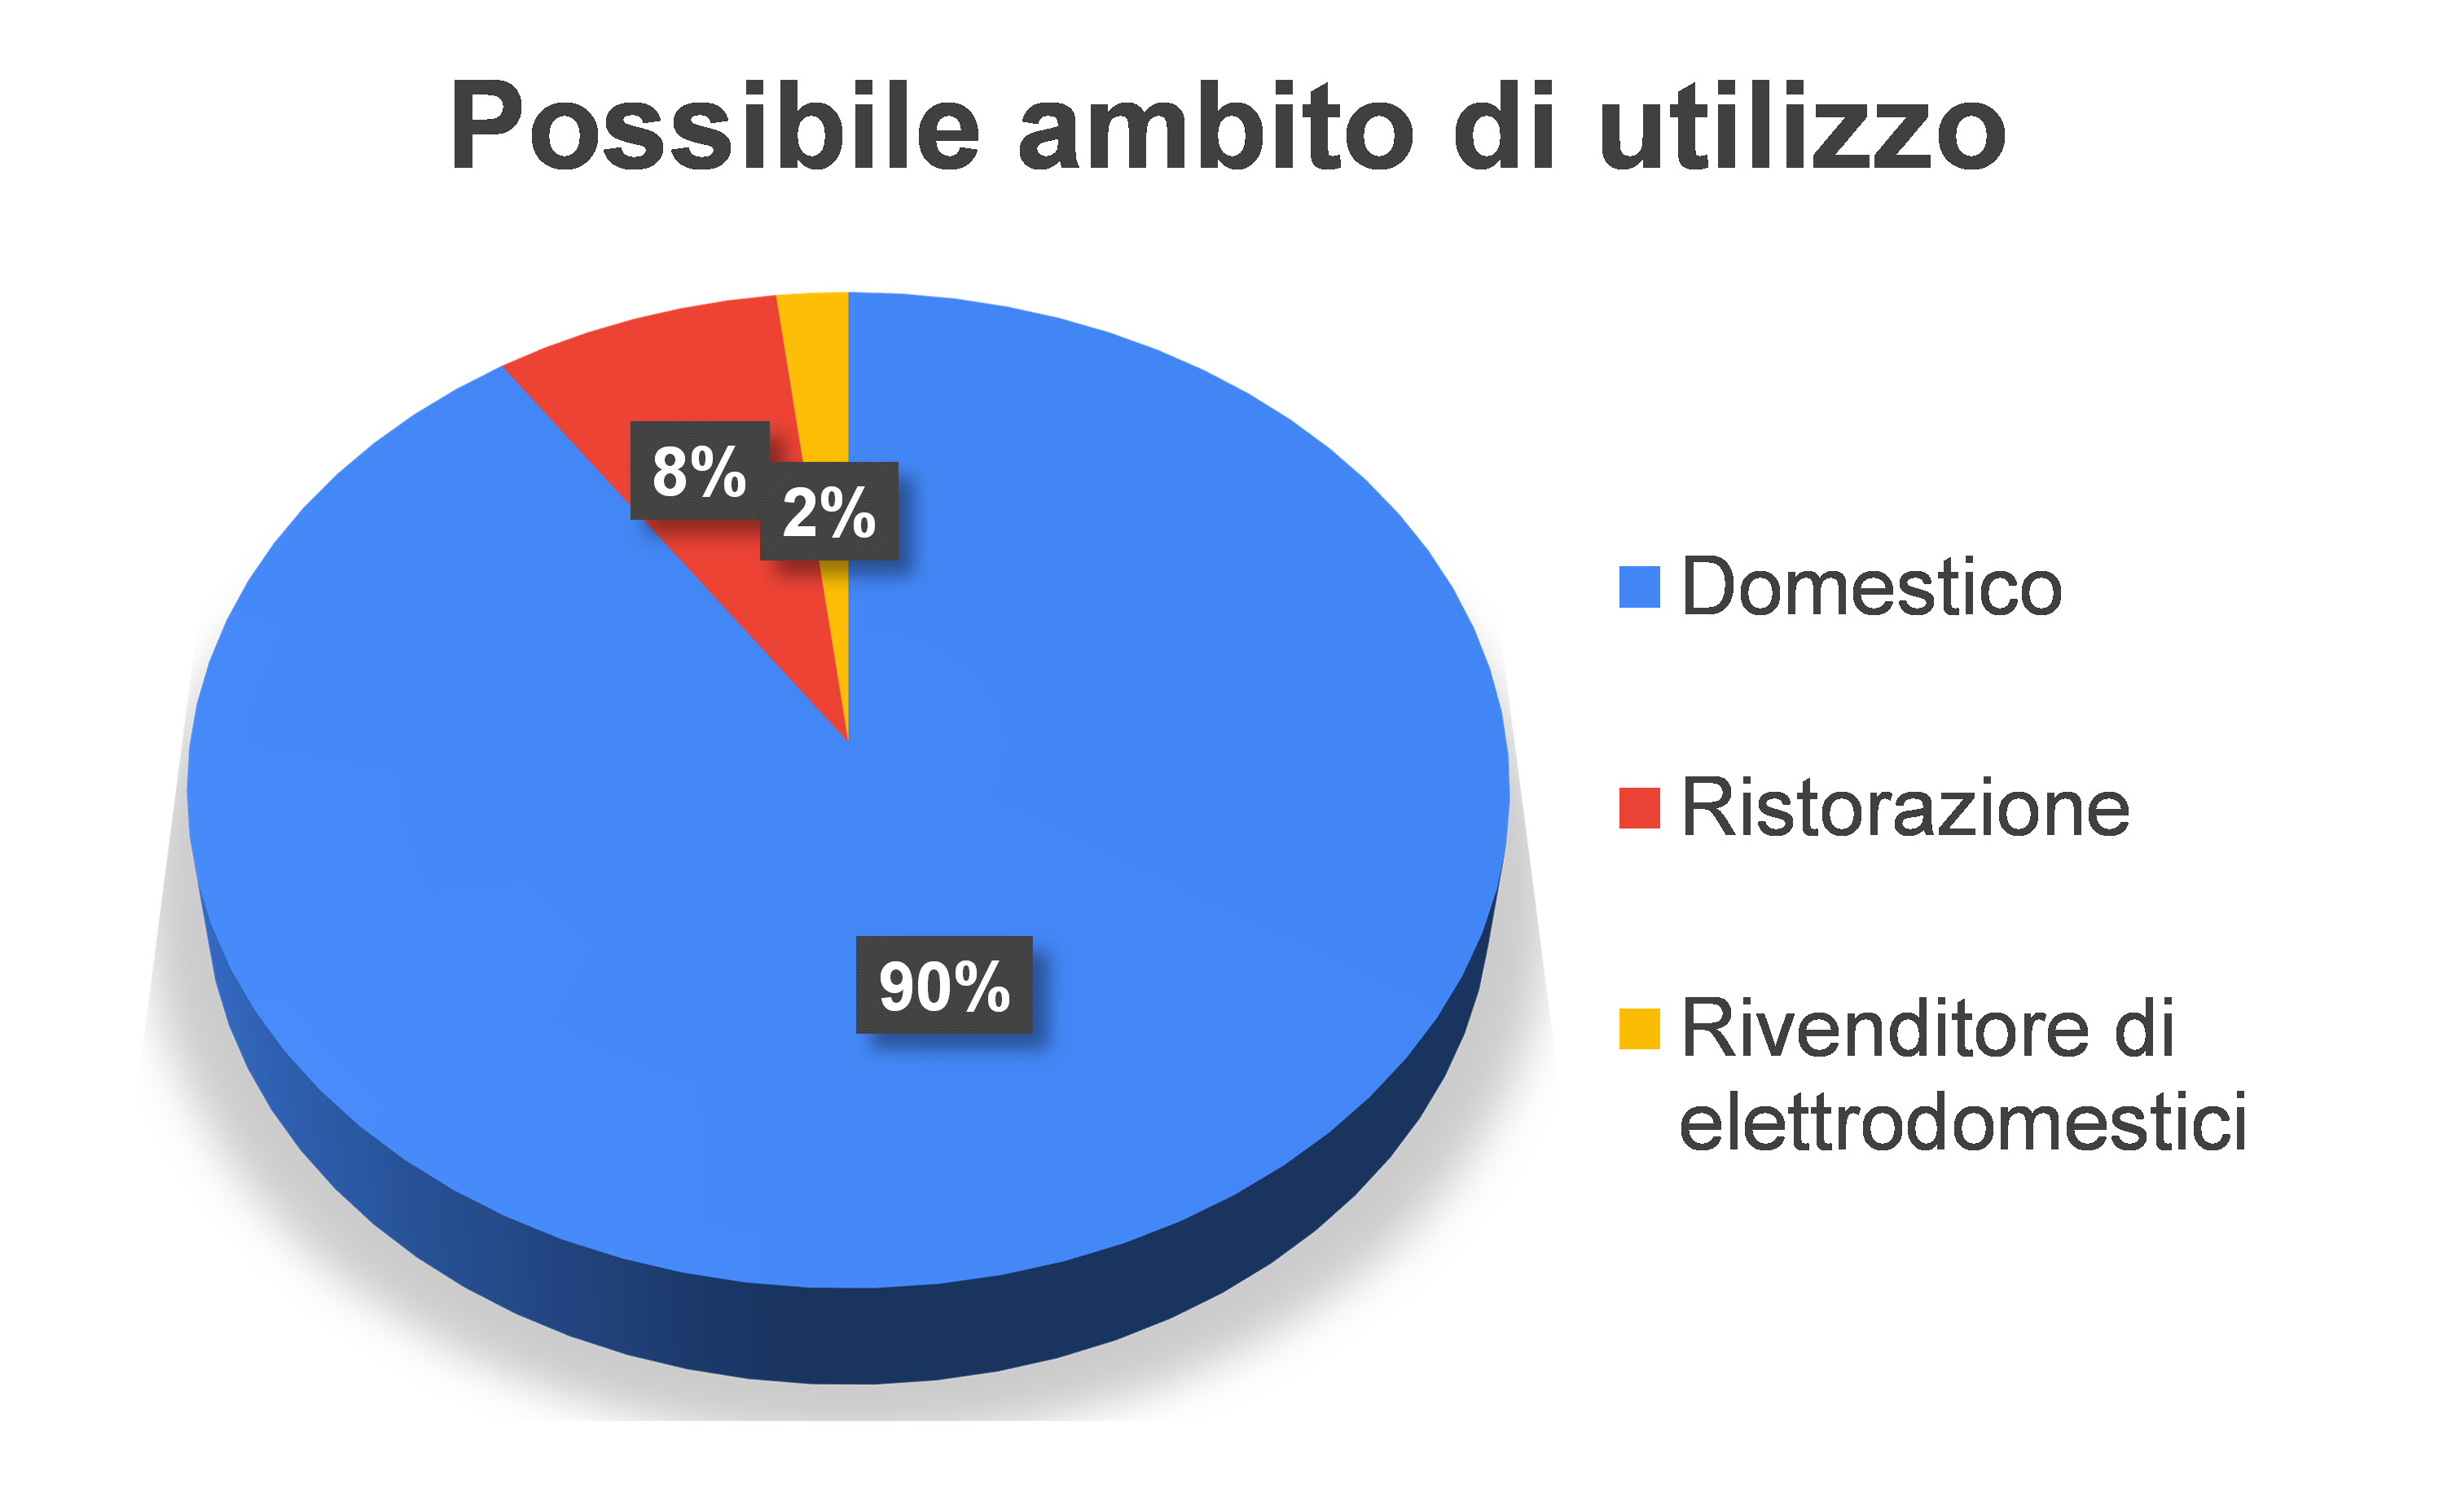
\includegraphics[width=\textwidth]{possibileUtilizzo.png}
    \caption{}
    \label{fig:possibile_utilizzo}
  \end{subfigure}
  \vskip\baselineskip
  \begin{subfigure}[b]{0.45\textwidth}
    \centering
    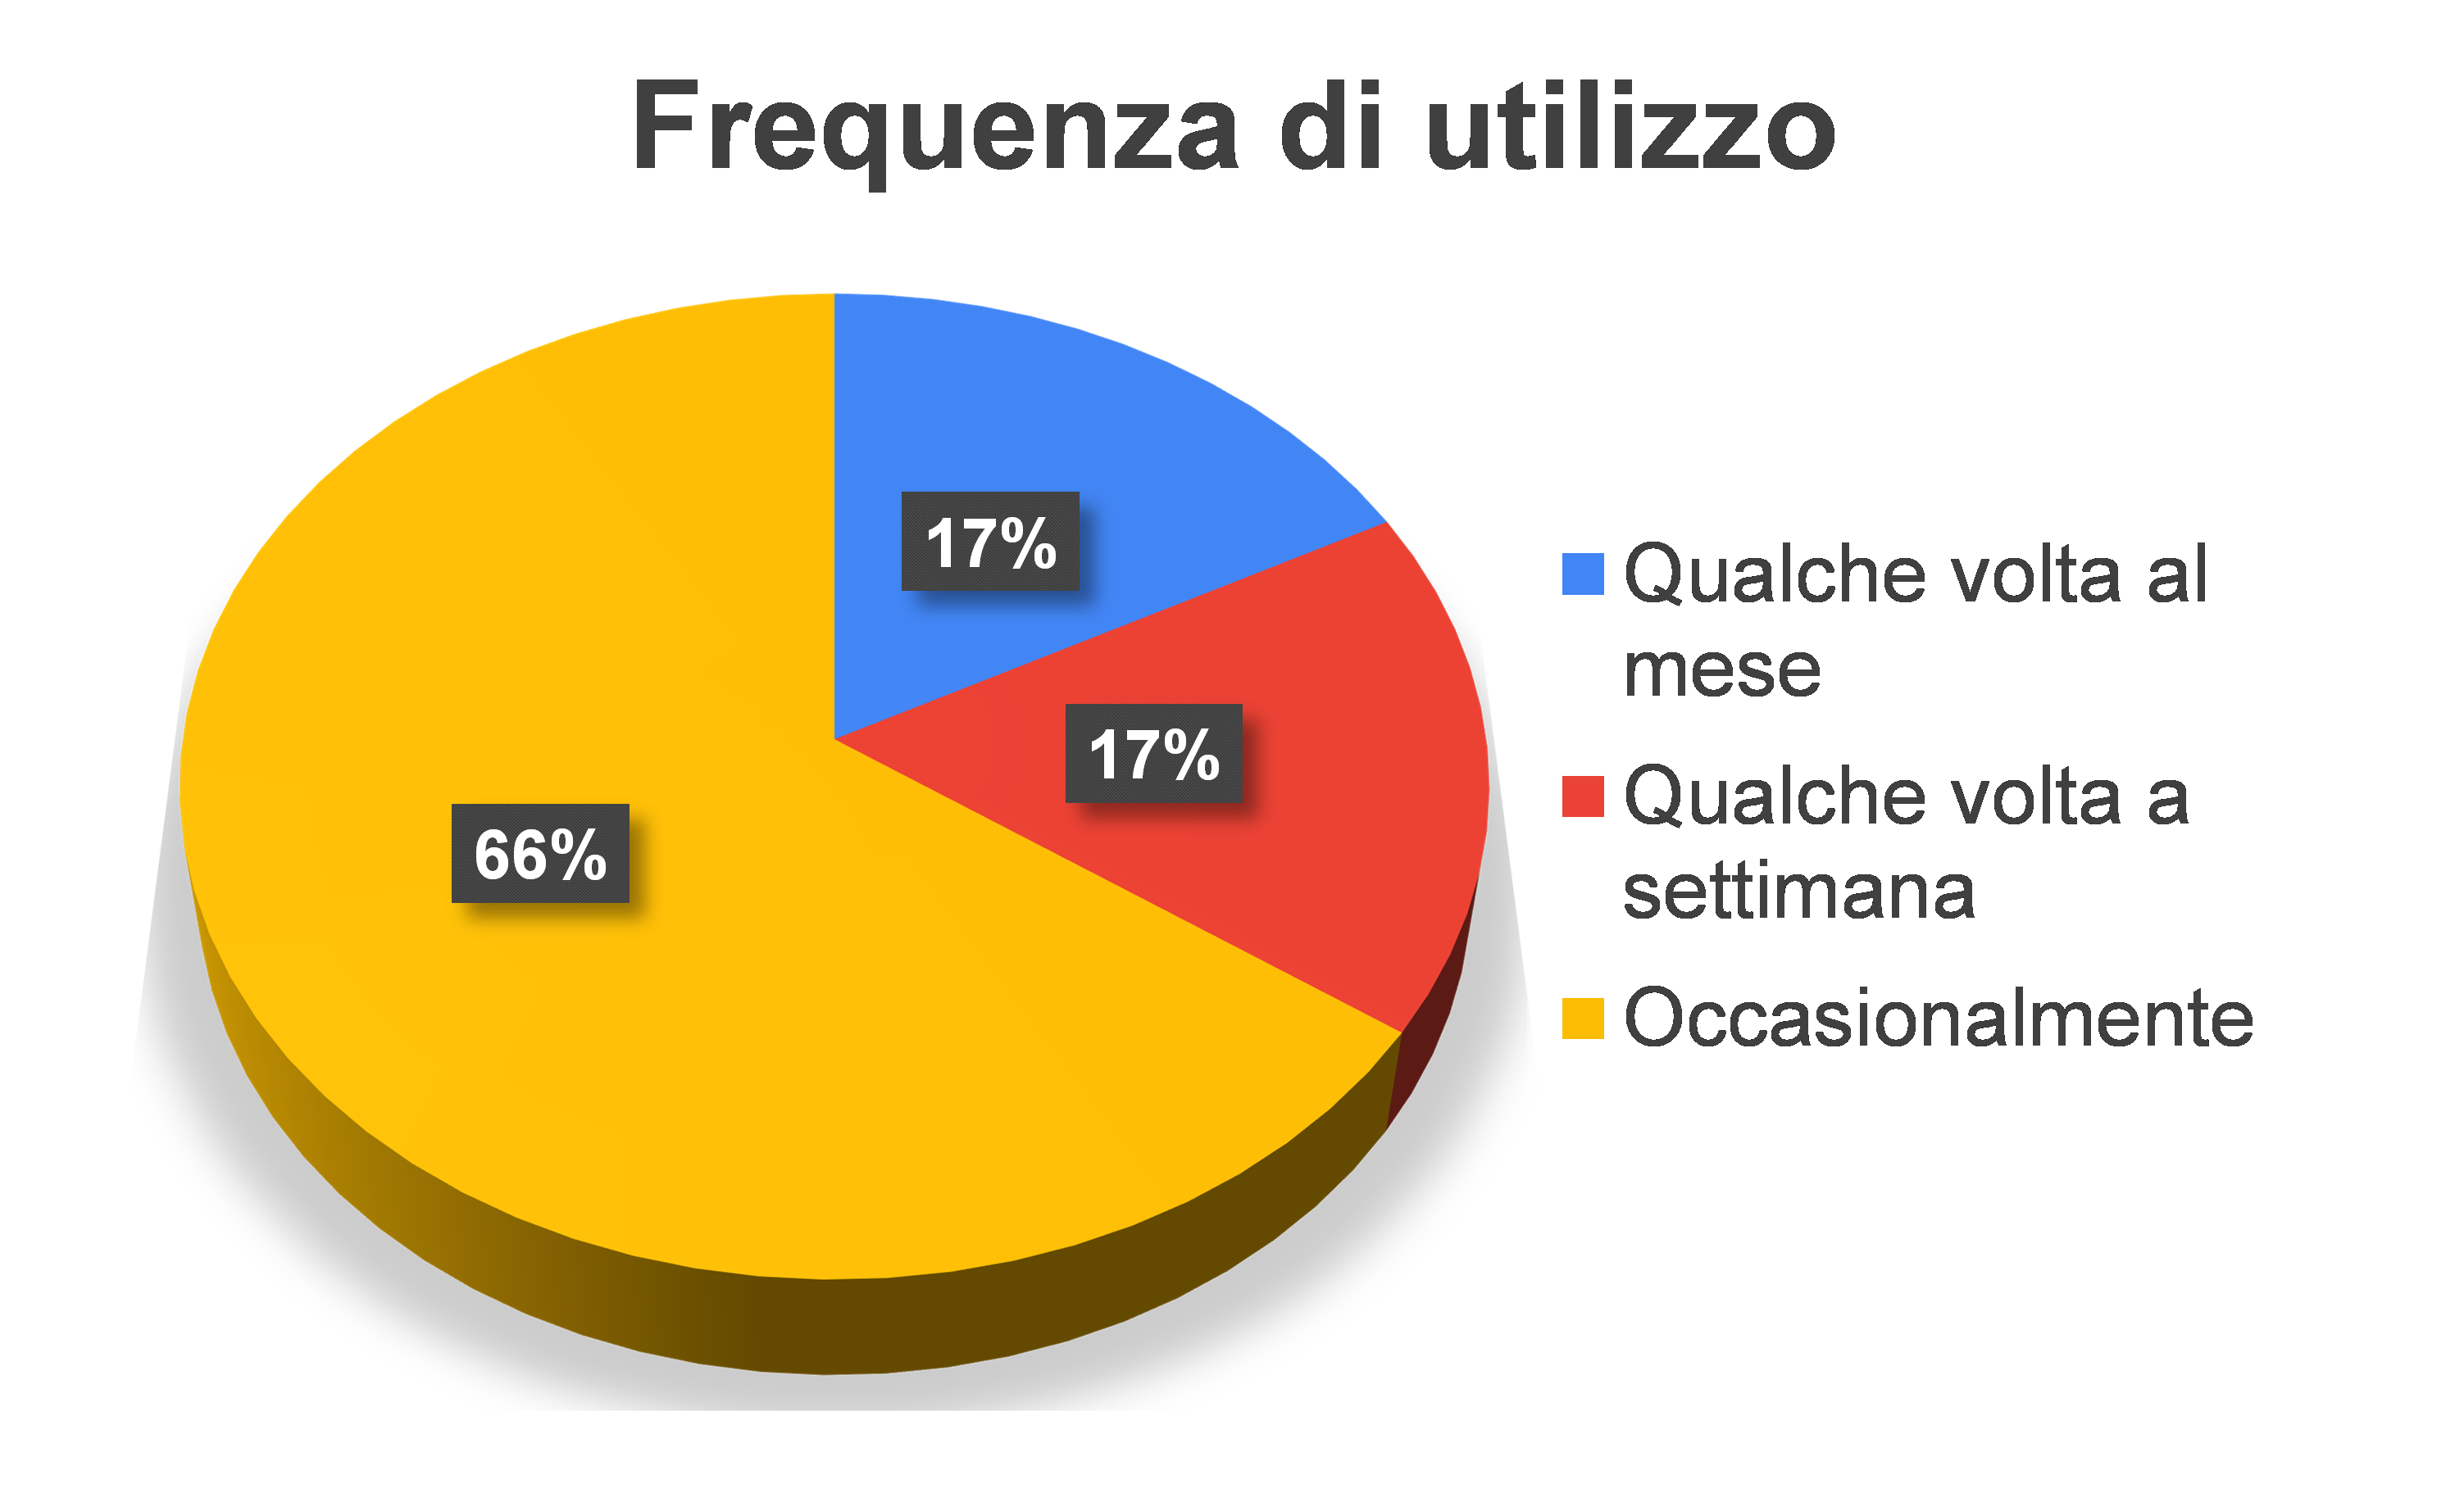
\includegraphics[width=\textwidth]{frequenzaUtilizzo.png}
    \caption{}
    \label{fig:frequenza_utilizzo}
  \end{subfigure}
  \caption{Conoscenza, possibile ambito di utilizzo e frequenza di utilizzo di un denocciolatore automatico}
  \label{fig:utilizzo_denocciolatore}
\end{figure}

\begin{figure}[H]
  \centering
  \begin{subfigure}[b]{\textwidth}
    \centering
    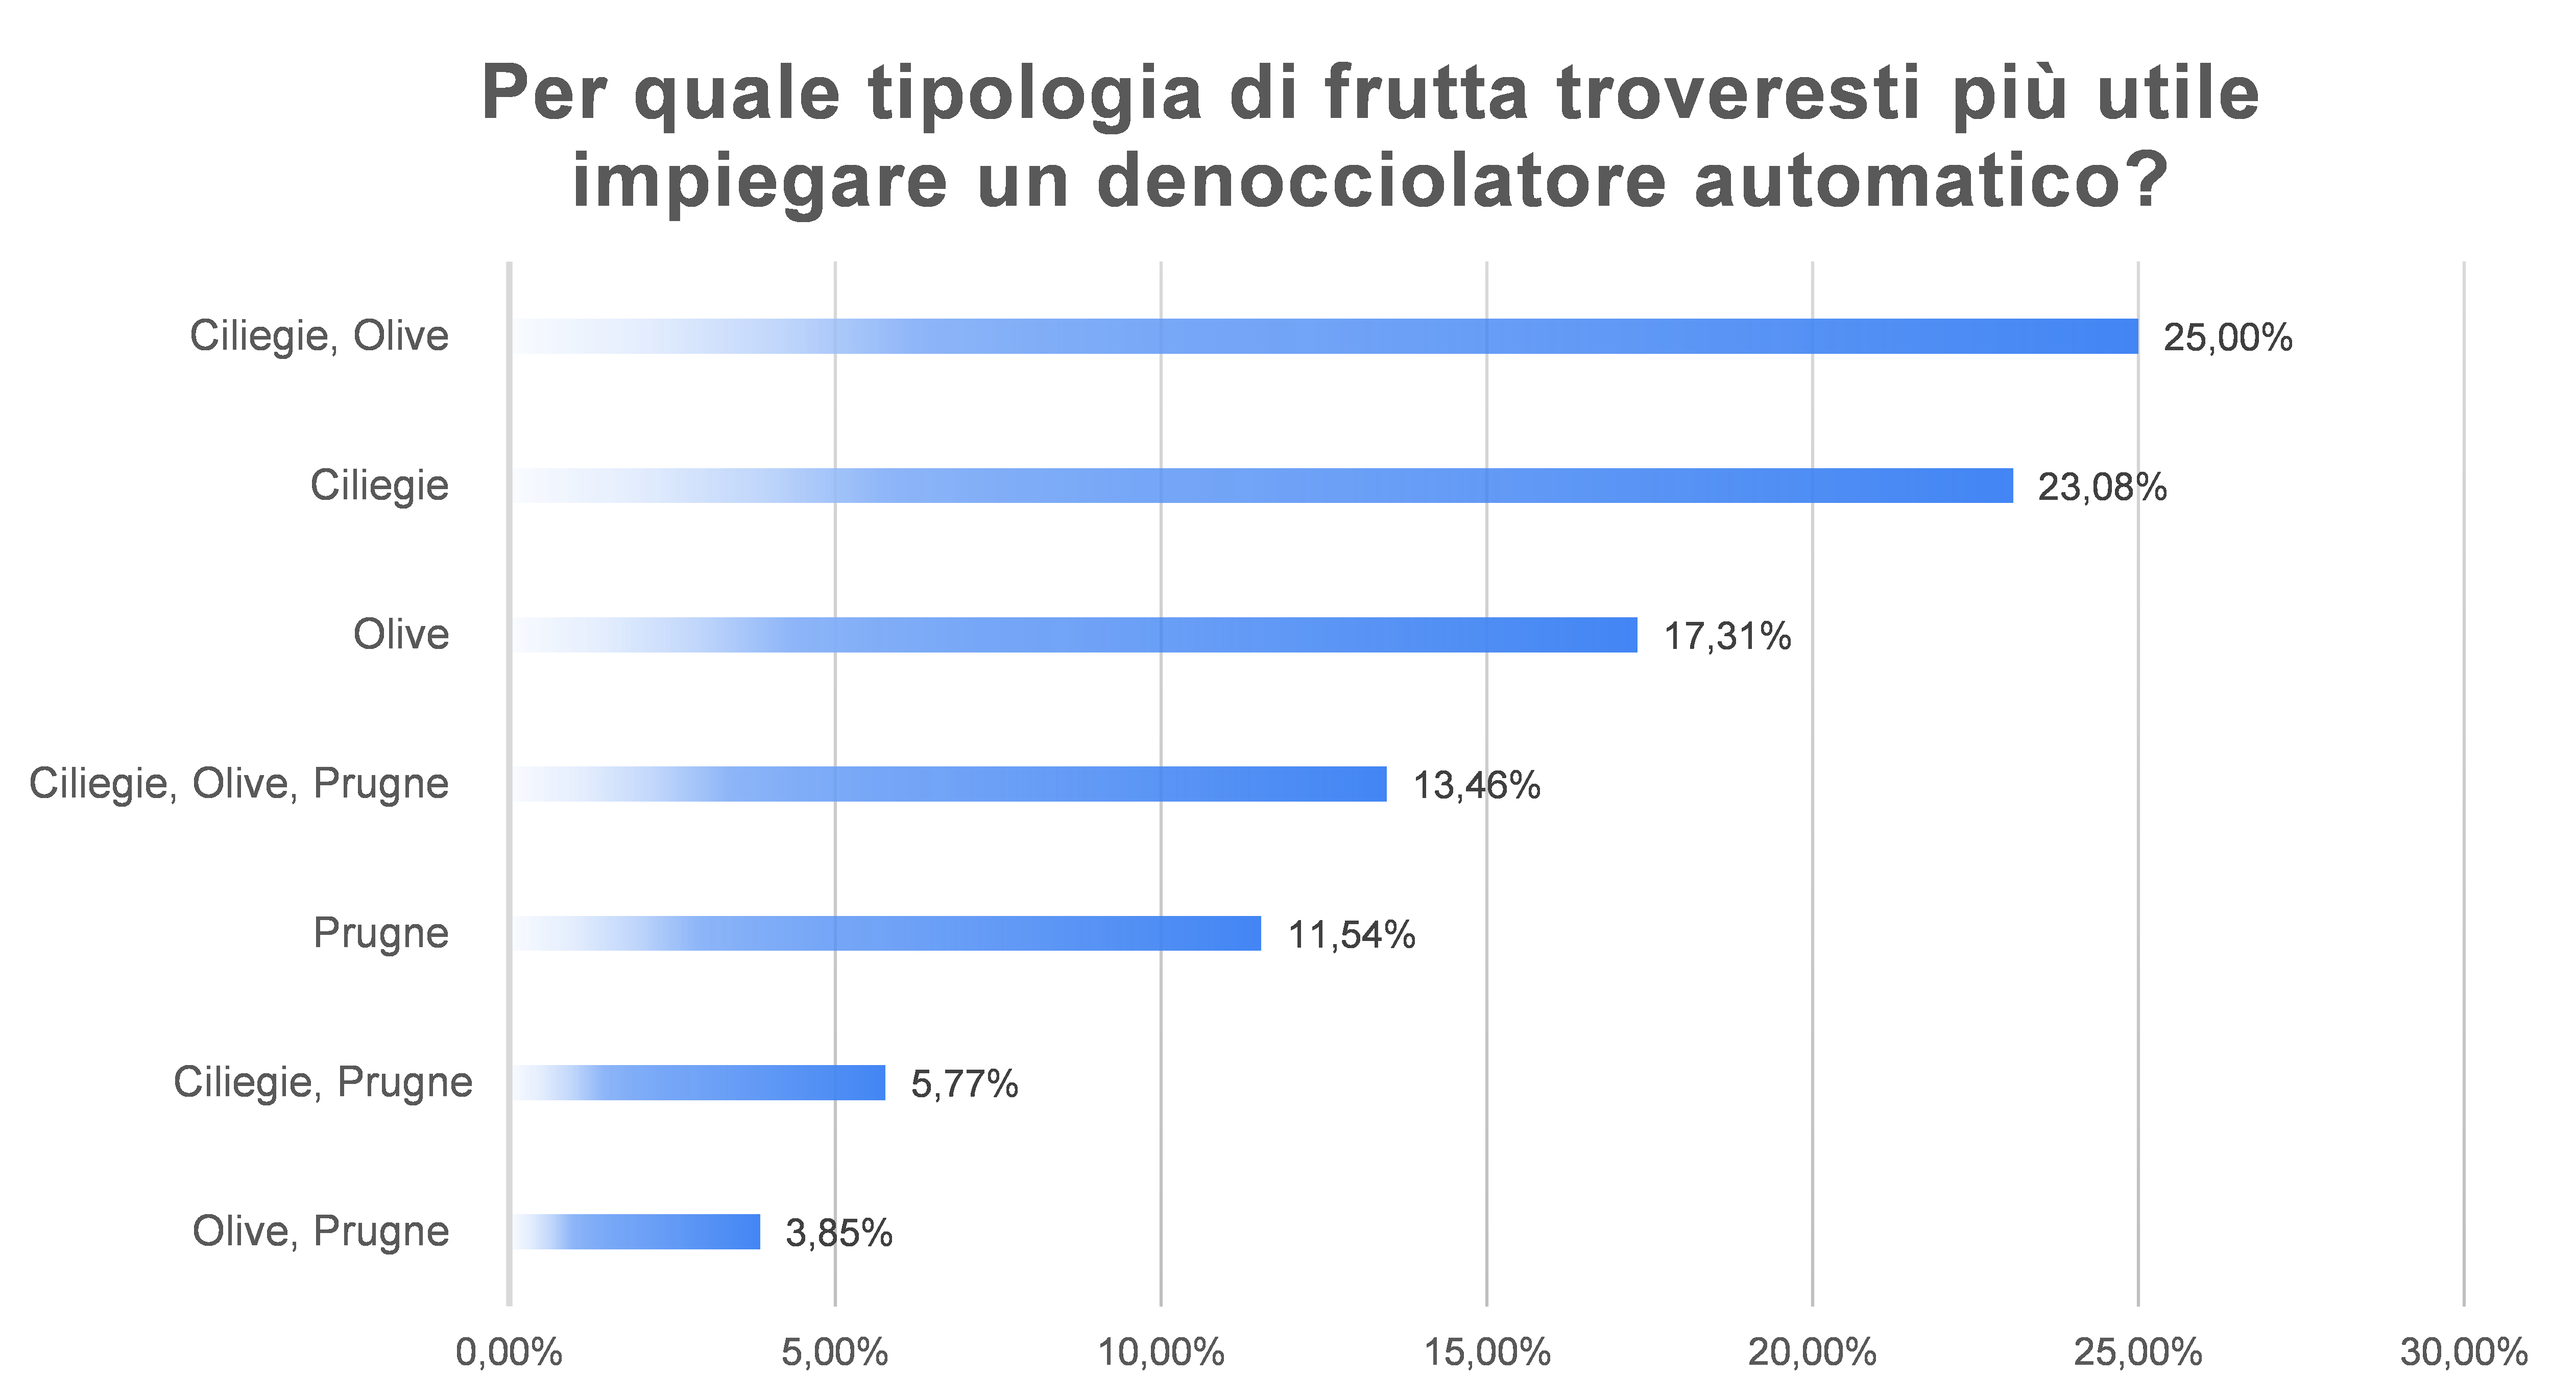
\includegraphics[width=\textwidth]{tipologiaFrutta.png}
    \caption{}
    \label{fig:tipologia_frutta}
  \end{subfigure}
  \vspace{0.5cm}

  \begin{subfigure}[b]{\textwidth}
    \centering
    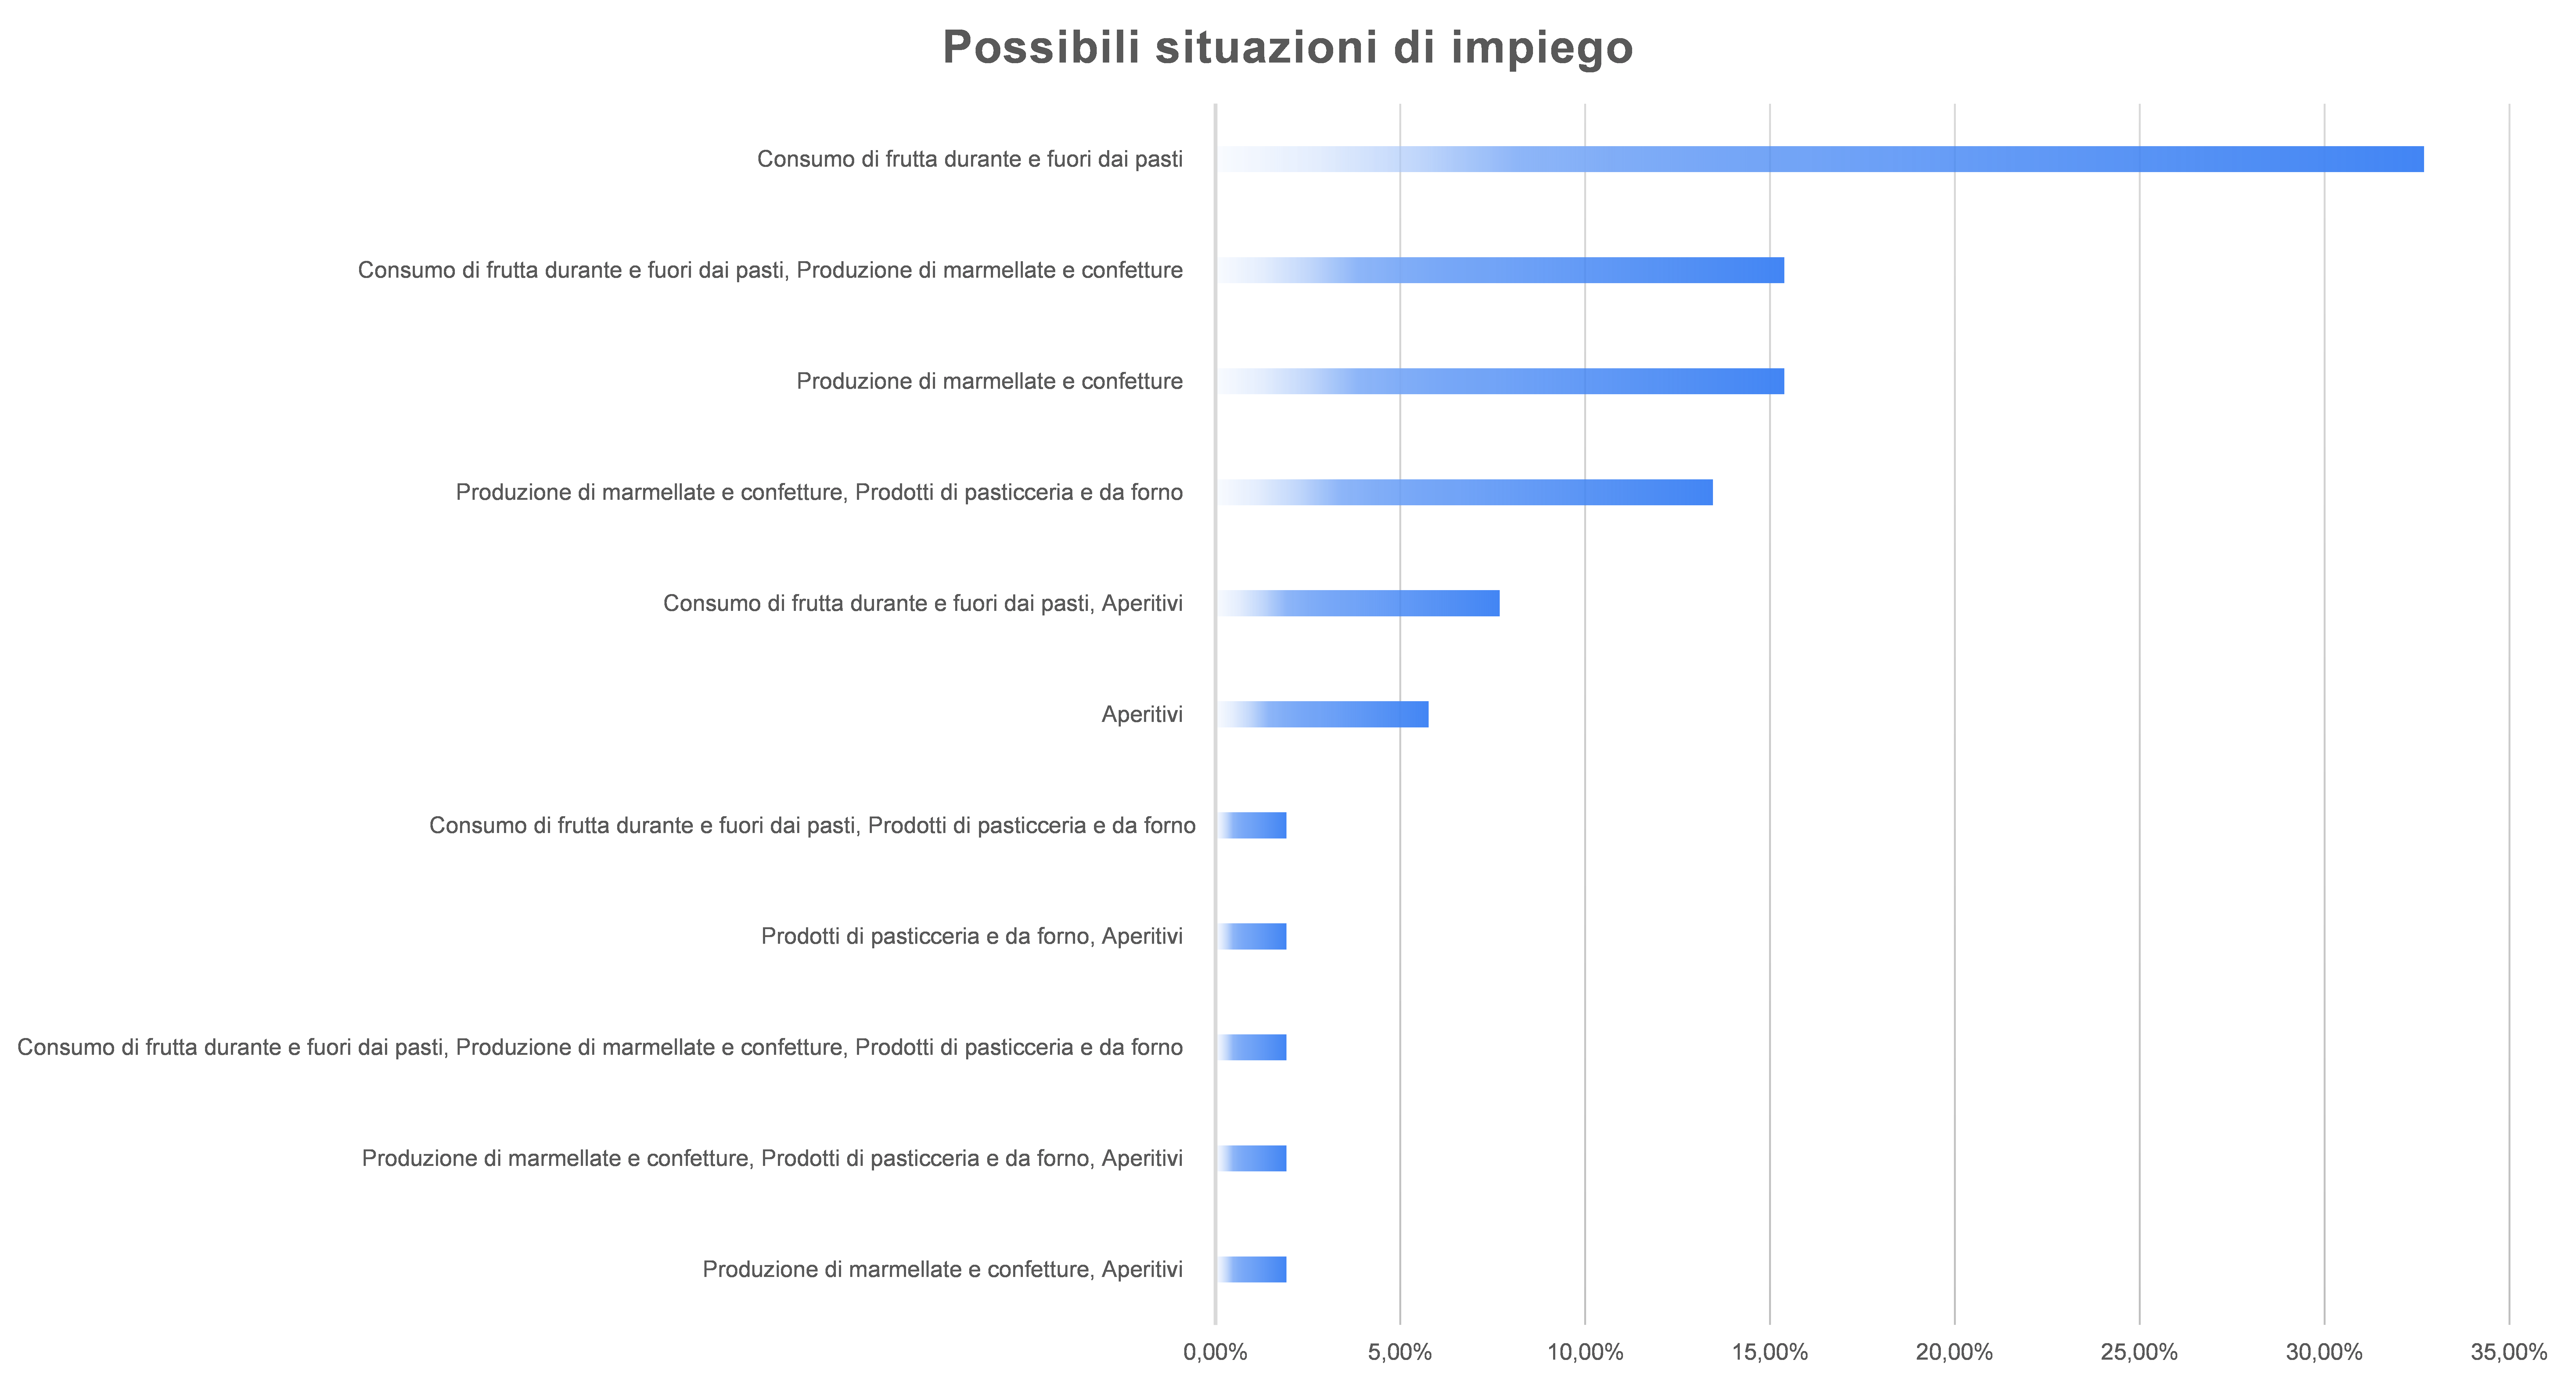
\includegraphics[width=\textwidth]{situazioniImpiego.png}
    \caption{}
    \label{fig:situazioni_impiego}
  \end{subfigure}

  \caption{Tipologia di frutti di maggiore interesse e utilizzo specifico}
  \label{fig:frutti_e_utilizzo}
\end{figure}

\newpage

\begin{landscape}
\begin{figure}
    \centering
    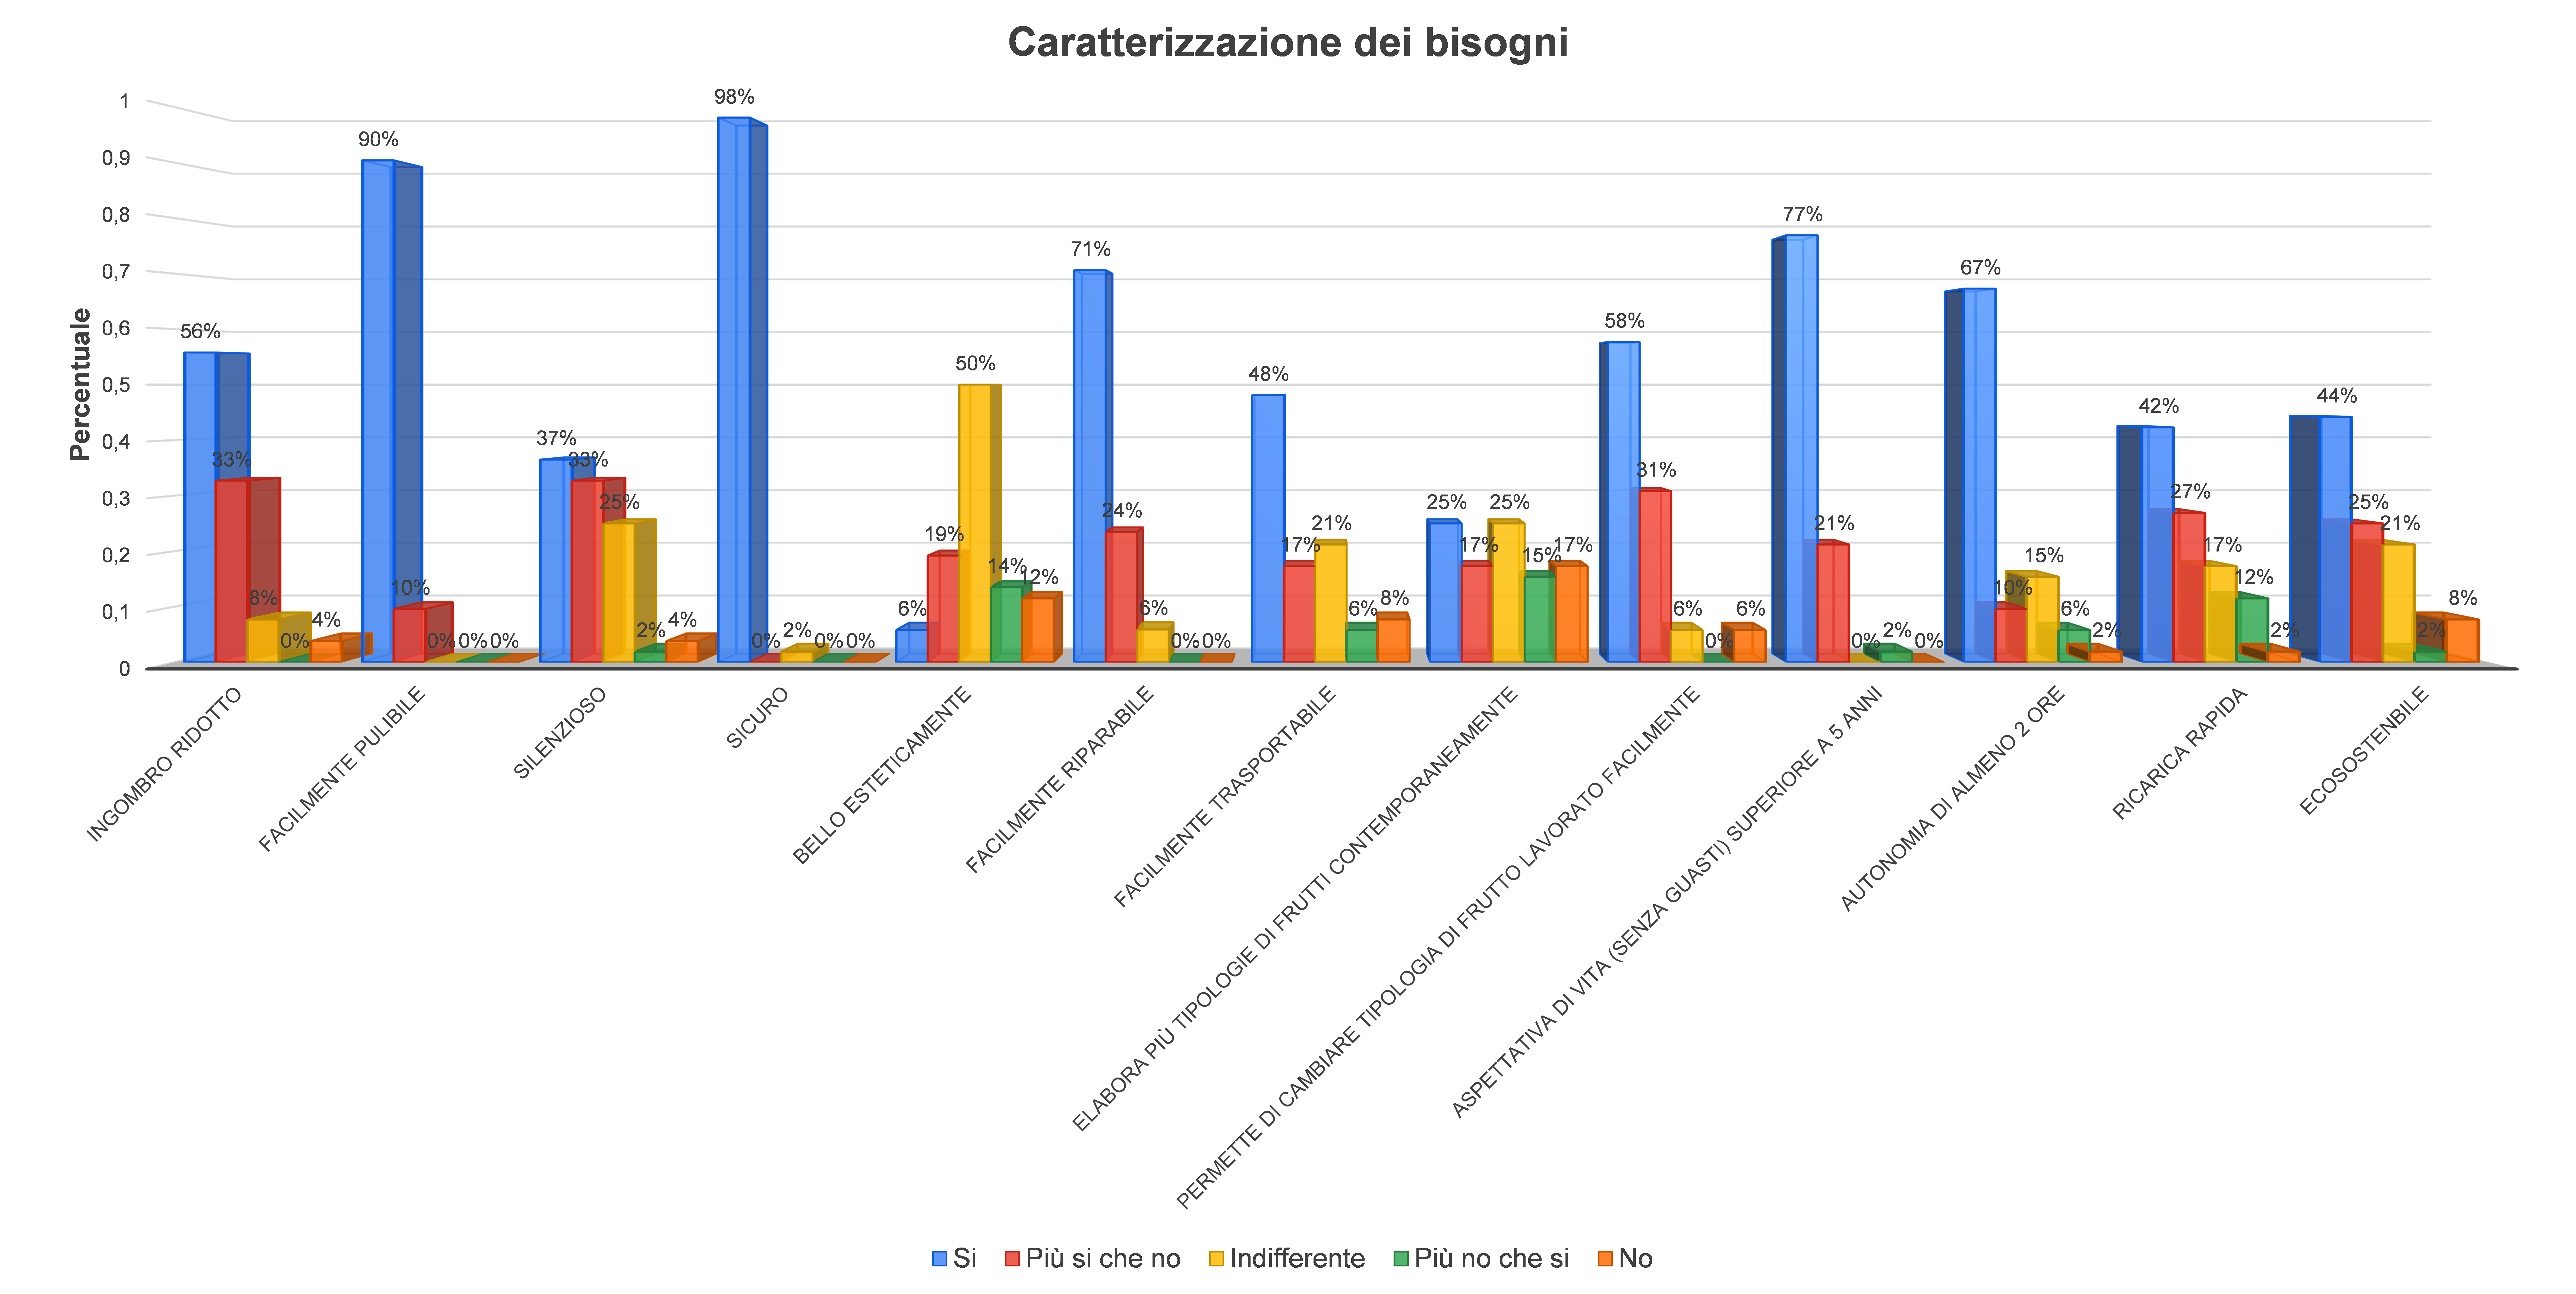
\includegraphics[width=1\linewidth]{caratterizzazioneBisogni.png}
    \caption{Caratterizzazione dei bisogni}
    \label{fig:caratterizzazioneBisogni}
\end{figure}
\end{landscape}

\newpage
Seguono le risposte fornite da alcuni partecipanti al sondaggio alla domanda opzionale "\textbf{Ci sono una o più caratteristiche e funzionalità che desidereresti ritrovare nel prodotto?}"
\begin{itemize}
\item \textit{Facilmente smontabile per la pulizia};
\item \textit{Ergonomico, efficiente, economico};
\item \textit{Ergonomia e facilità di utilizzo. Mi aspetto che possa essere utilizzato anche da signori anziani, quindi deve essere comodo e pratico};
\item \textit{Materiali come plastiche resistenti o acciaio inossidabile per allungare la vita del prodotto. La facilità di pulizia per me è fondamentale in quanto usandolo occasionalmente va ripulito bene prima di riporlo. Potrebbe anche essere alimentato dalla linea tramite spina elettrica e non ricaricabile};
\item \textit{Componenti rimovibili lavabili in lavastoviglie};
\item \textit{Poter inserire tutti i frutti che voglio lavorare all’inizio e poter allontanarmi dalla macchina mentre è in funzione, con segnale acustico per avvisarmi quando finisce il processo di lavorazione};
\item \textit{Praticità}.
\end{itemize}

\section{Interpretazione dei risultati}
Dai grafici presenti in Figura~\ref{fig:utilizzo_denocciolatore} si evince che la maggior parte della popolazione campionata non ha mai utilizzato un denocciolatore ma comunque è a conoscenza del tipo di oggetto o ne ha sentito parlare. Inoltre dalla Figura~\ref{fig:possibile_utilizzo}  si deduce come l'utilizzo più possibile sia quello domestico e la maggioranza della popolazione utilizzerebbe il denocciolatore con frequenza occasionale (66\%, come riportato in Figura~\ref{fig:frequenza_utilizzo}). 

Dal sondaggio inoltre emerge come la popolazione campionata sia particolarmente interessata ad utilizzare il denocciolatore automatico per ciliegie e olive (Figura~\ref{fig:tipologia_frutta}). Per quanto riguarda le possibili situazioni di impiego, il consumo di frutta durante e fuori dai pasti e la produzione di marmellate e confetture sono state scelte maggiormente dalla popolazione campionata (Figura~\ref{fig:situazioni_impiego}).

In Figura~\ref{fig:caratterizzazioneBisogni} sono riportati i risultati della caratterizzazione dei bisogni. Dal grafico si evince come per la popolazione campionata siano molto importanti la facilità di pulizia, la sicurezza, l'aspettativa di vita (senza guasti) superiore a 5 anni, l'autonomia di almeno 2 ore e la rapidità nel cambio della tipologia di frutto lavorato. Al contrario non risultano avere particolare importanza l'aspetto estetico e la possibilità di lavorare più tipologie di frutti contemporaneamente (ossia elaborare più frutti diversi contemporaneamente).

\section{Definizione delle specifiche obiettivo e costruzione della Casa della Qualità}
In questa sezione verrà illustrato il procedimento che porta alla definizione delle specifiche obiettivo, ovvero dei valori misurabili attribuiti alle metriche che il gruppo si prefigge di raggiungere nel prodotto finale e che si suppone possano fornire un vantaggio competitivo al prodotto. Infine si procede alla costruzione della Casa della Qualità.
\subsection{Definizione dei bisogni cliente}
Sulla base dei risultati ottenuti dal sondaggio riportati in Sezione \autoref{sec:identificazioneBisogniCliente} ed a seguito di un'approfondita analisi di gruppo, si sono definiti i bisogni riportati nella tabella in Figura~\ref{fig:bisogni}. Ad ogni bisogno individuato è stato attribuito un valore di importanza variabile tra 1-3-5, dove 1 corrisponde ad importanza minore mentre 5 corrisponde ad importanza maggiore.
\begin{figure}[H] %[H] serve a forzare l'immagine nella posizione devo metto il codice
    \centering
    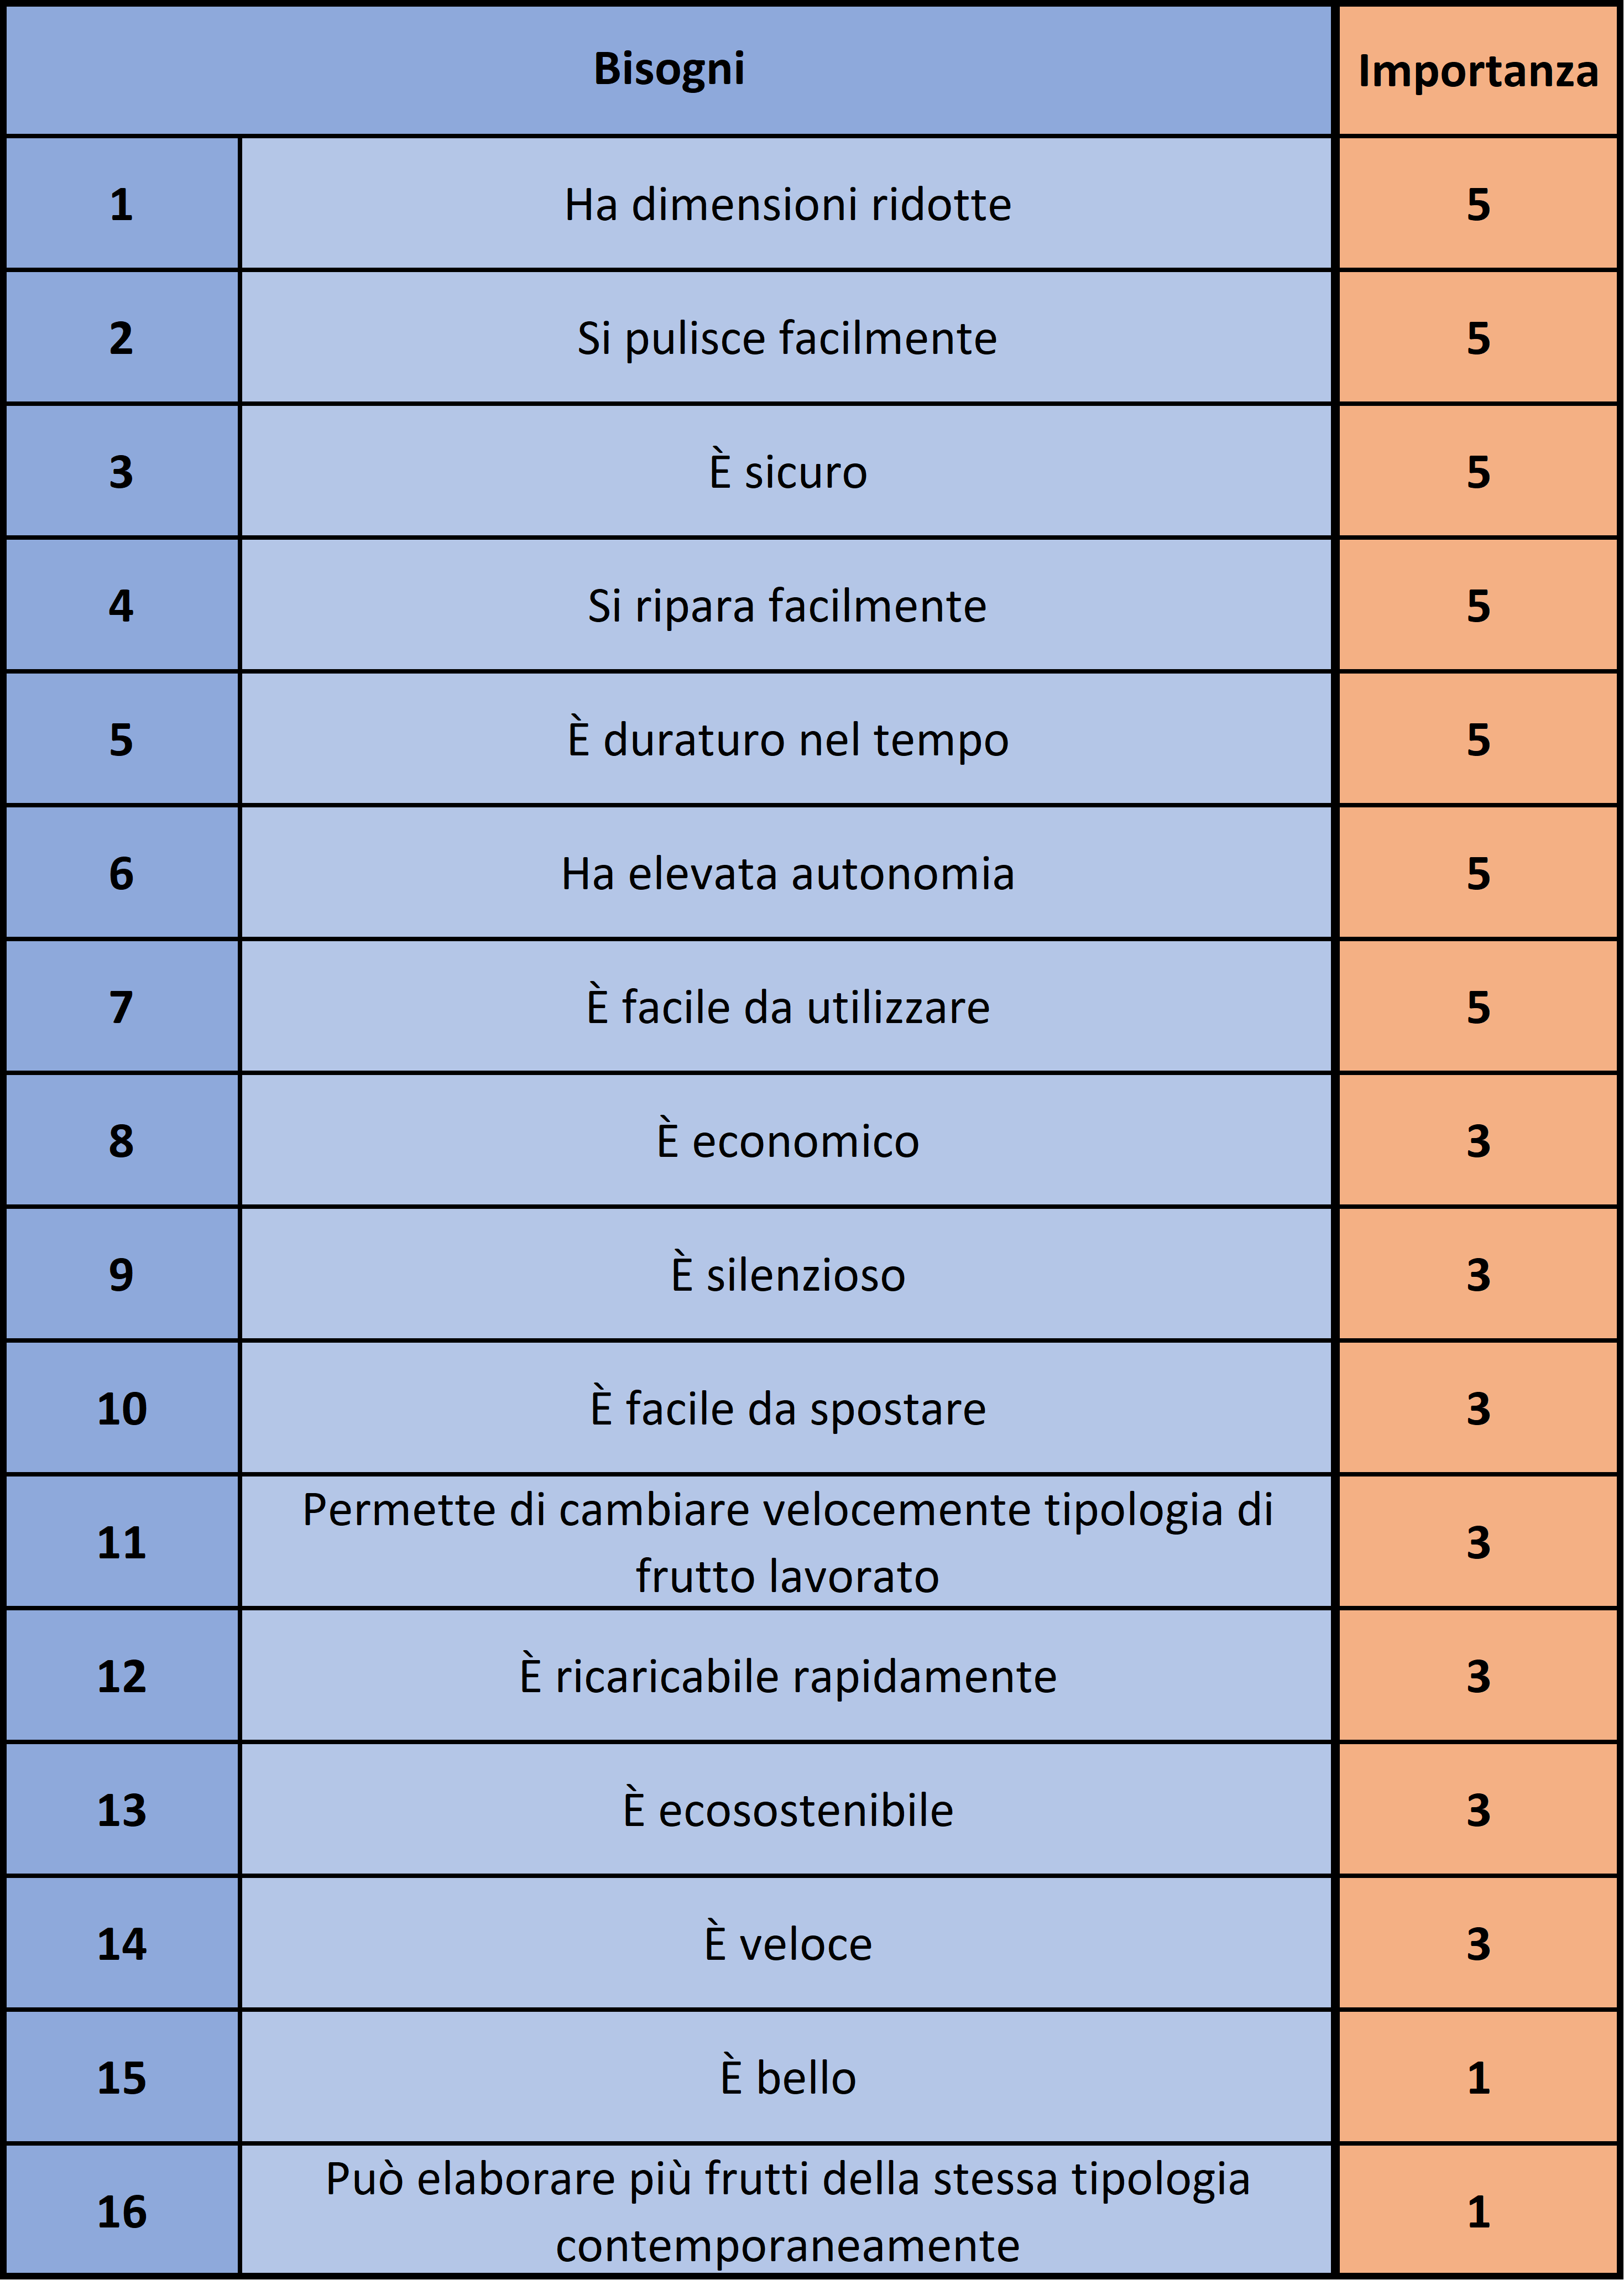
\includegraphics[width=0.65\linewidth]{1bisogni.png}
    \caption{Bisogni individuati e relative importanze}
    \label{fig:bisogni}
\end{figure}

\newpage

\begin{landscape}
\begin{figure}
    \centering
    \includegraphics[width=1\linewidth]{8casaQualitàV2.png}
    \caption{Casa della Qualità}
    \label{fig:casaQualità}
\end{figure}
\end{landscape}

\newpage


\section{Identificazione e ordinamento delle sottofunzioni}

\begin{itemize}
\item Ricezione ed accumulo di energia;
\item Logica di controllo;
\item Rilevamento sicurezza;
\item Fault check;
\item Selezione della tipologia di frutto da lavorare;
\item Inserimento dei frutti nel macchinario;
\item Orientamento del frutto;
\item Veicolazione del frutto;
\item Conversione dell'energia elettrica in energia meccanica;
\item Conversione del moto rotatorio in moto alterno;
\item Rimozione del nocciolo dal frutto;
\item Veicolazione del nocciolo;
\item Veicolazione della polpa;
\item Espulsione del nocciolo;
\item Espulsione della polpa.
\end{itemize}

\end{document}
% PR fittizia per abilitare i commenti su main.tex

